
\chapter{Theoretical Framework}
This chapter provides the theoretical foundation required to understand the work presented in this thesis. It is organized into several sections, each covering a key topic relevant to the design and implementation of the F-engine for CHARTS. The chapter begins with an introduction to radio astronomy fundamentals, followed by a description of time domain astronomy and transient astronomical phenomena such as fast radio bursts and pulsars, including their main propagation effects. Next, it reviews essential concepts in digital signal processing, including sampling, quantization, filtering, polyphase filterbanks, and frequency analysis using the discrete Fourier transform. The chapter then discusses spectrometers and correlators, outlining their main types, performance metrics, and typical architectures. Finally, it presents an overview of the computational hardware used, with a focus on field programmable gate arrays and their integration with other processing units, such as GPUs, via high-speed optical interconnects. Also included is a description of the Xilinx AMD RFSoC 4x2 platform, which serves as the basis for the F-engine developed in this work.

\section{Radio astronomy fundamentals}
\label{sec:radio_fundamentals}
Radio astronomy, as its name suggests, is the branch of astronomy dedicated to observing celestial phenomena in the radio spectrum. The radio domain, as shown in Figure \ref{fig:radio_spectrum}, encompasses a substantial portion of the electromagnetic spectrum, spanning from kilometer wavelengths to mm/sub mm wavelengths\footnote{Here microwaves are considered a subset of the radio spectrum.}. From the ground, however, observations are limited to the so-called radio window, which spans approximately from $\sim10$~MHz to just below $\sim1$~THz in very dry places.
This broad range, spans nearly five orders of magnitude in frequency and encompasses a wide variety of physical emission mechanisms. Virtually all astronomical objects emit radio waves, which, unlike higher-frequency radiation, can penetrate dense gas and interstellar dust \citep{essential_radio_astronomy}. As a result, radio observations rarely suffer from obscuration and have revealed a rich universe of phenomena, including radio galaxies, quasars, pulsars, radio transients, cold molecular clouds, the cosmic microwave background, cosmic magnetic fields, etc.
\begin{figure}[h!]
	\centering
	\includegraphics[width=\textwidth]{tikz figures/build/em_spectrum.pdf}
	\caption[Electromagnetic spectrum overview]{Overview of the electromagnetic spectrum, showing the relationship between wavelength ($\lambda$), frequency ($\nu$), and photon energy ($E=h\nu$). The spectrum is divided into regions such as radio, microwave (subset of radio), infrared (IR), ultraviolet (UV), X-ray, and gamma rays. The corresponding frequency and energy scales are indicated, along with common units for each region. Adapted from \href{https://tikz.net/electromagnetic_spectrum/}{TiKz.net}, Izaak Neutelings.}
	\label{fig:radio_spectrum}
\end{figure}

The accessibility of the radio spectrum from the ground is made possible by the Earth’s atmosphere, which is transparent across certain wavelength ranges but opaque in others. Figure \ref{fig:atmospheric_windows} illustrates the main atmospheric transmission windows. In the radio domain, the lower boundary of observability is set by the ionosphere, which reflects radiation below $\sim10$~MHz, while signals below $\sim2$~MHz are absorbed by the ionized interstellar medium. The upper boundary is less sharply defined and extends into the mm/sub mm regime, where water vapor and the troposphere strongly absorb radiation. Despite these limitations, radio waves penetrate the atmosphere more effectively than most other bands, making ground-based radio astronomy particularly powerful.
\begin{figure}[h!]
	\centering
	\includegraphics[width=0.8\textwidth]{../figures/atmospheric_transmission.png}
	\caption[Atmospheric transmission]{Atmospheric transmission as a function of wavelength. The graph shows the percentage of electromagnetic radiation that passes through Earth's atmosphere across different wavelength ranges. Gray areas represent regions of high opacity where radiation is mostly blocked, while clear areas indicate atmospheric windows where observations are possible. Several radio telescopes and antennas are illustrated at various positions corresponding to their operating wavelengths. The radio window (from $\sim1$ mm to $\sim10$ m) and visible light window (from $\sim400$ nm to $\sim700$ nm) are prominent atmospheric transmission windows, while other regions like ultraviolet, far infrared, and parts of the microwave spectrum experience significant absorption. Image taken from \citet{essential_radio_astronomy}.}
	\label{fig:atmospheric_windows}
\end{figure}

Although space-based observatories have expanded access to the entire electromagnetic spectrum, radio astronomy continues to offer distinct advantages. Because radio photons carry very low energies, they can be coherently amplified while preserving phase information, something unattainable at higher frequencies, where quantum noise dominates (see \citealt{RevModPhys.82.1155} for detailed discussion of quantum noise). This property makes it possible to build highly sensitive, multi-element interferometers that achieve angular resolutions and astrometric precision far beyond those of other wavelength regimes. In addition, radio signals can be digitized with exceptional spectral resolution and frequency accuracy, enabling advanced techniques such as aperture synthesis and \gls{vlbi}. These methods allow astronomers to image sources with angular resolutions down to the order of \si{\micro\arcsec}, as exemplified by the $\sim\SI{20}{\micro\arcsec}$ image of the M87 black hole produced by \cite{Akiyama_2019}.
\subsection{Relevant quantities in radio astronomy}
In radio astronomy, several fundamental quantities are required to describe and interpret the emission from astrophysical sources. These quantities connect the intrinsic radiation properties of the source with the signal detected by a radio telescope, which is affected by distance, frequency range and the telescope's characteristics such as aperture size and efficiency.


The first quantity to be defined is the specific intensity ($I_\nu$), which represents the received emission. It is defined as the power received per unit area, frequency, and solid angle:
\begin{equation}
	I_\nu \;=\; \frac{\mathrm{d}P}{ (\cos\theta \, \mathrm{d}\sigma) \, \mathrm{d}\Omega \, \mathrm{d}\nu}
\end{equation}
where $\theta$ is the angle between the direction of the radiation and the observer's line of sight, $\mathrm{d}\sigma$ is the area element on the telescope surface, $\mathrm{d}\Omega$ is the solid angle element of the source, and $\mathrm{d}\nu$ is the frequency element. It is important to note that the specific intensity is an intrinsic property of the source, while the received power depends on the distance and the characteristics of the telescope.


Building on the concept of specific intensity, it is essential to understand how thermal emission from astrophysical sources is described. At the beginning of the 20th century, Planck introduced the idea that electromagnetic radiation is emitted in discrete energy packets\footnote{Although Planck is historically credited with introducing the concept of energy quantization in \emph{quanta}, when he first formulated his radiation law, he regarded the discretization of energy as a mathematical trick rather than a fundamental physical principle. In fact, Planck himself did not initially believe that energy was inherently quantized; he considered it a pragmatic approach to fit experimental data, a ``desperate measure" in his own words (see \citealt{Planck1949-PLASAA-3} autobiography), to make his theory consistent with observations. Luckily, his conviction that the laws of thermodynamics should hold at all costs led him to stick to the idea of quantized energy levels.
}, or \emph{quanta}, laying the foundation for quantum theory and revolutionizing the understanding of blackbody radiation. The spectral brightness, which shares the same units as specific intensity, quantifies the power emitted per unit area, solid angle, and frequency by a blackbody at temperature $T$. This relationship is mathematically expressed by Planck's law \citep[see][Chapter~7]{StatisticalMechanics}:
\begin{equation}
	B_\nu(\nu, T) = \frac{2h\nu^3}{c^2} \frac{1}{e^{h\nu/kT}-1}
	\label{eq:planck}
\end{equation}
where $h$ is Planck's constant, $c$ is the speed of light, and $k$ is Boltzmann's constant. Planck's law has two notable limiting cases: at high frequencies ($h\nu \gg kT$), it reduces to Wien's law, while at low frequencies ($h\nu \ll kT$), it approaches the Rayleigh-Jeans approximation. 
Figure \ref{fig:spectral_brightness} illustrates the spectral brightness $B_\nu$ as a function of frequency\footnote{It is important to clarify that $B_\nu(\nu,T)$ and $B_\lambda(\lambda,T)$ are distinct quantities with different units, \si{\watt \per \steradian  \per \meter \squared \per \hertz} and \si{\watt \per \steradian \per \meter \cubed}, respectively. The conversion between them is given by $B_\nu = \frac{c}{\nu^2} B_\lambda$.} 
for a blackbody at 5500~K (approximately the temperature of the Sun's surface). The plot compares the predictions of Planck's law, the Rayleigh-Jeans approximation, and Wien's law, where the limiting behaviors are evident. Particularly the spectral brightness in the radio regime (below $\sim 10^{12}$ Hz) appears as a straight line in this log-log plot, indicating the validity of the Rayleigh-Jeans approximation in this frequency range.
\begin{figure}[h!]
	\centering
	\includegraphics{../figures/blackbody_radiation_frequency.pdf}
	\caption[Blackbody radiation example]{Relationship between spectral brightness and frequency for a blackbody at 5500 K, where the visible spectrum is highlighted in the rainbow and the peak radiation is achieved. The predictions of Planck's law, Rayleigh-Jeans approximation, and Wien's law are shown.}
	\label{fig:spectral_brightness}
\end{figure}

If the radiation is in a Local Thermodynamical Equilibrium (LTE), the intensity behaves exactly as a blackbody (Eq. \ref{eq:planck}), $(I_\nu)_{\text{LTE}} \rightarrow B_\nu(T)$.
From this relationship and Planck's law given in Eq. \ref{eq:planck}, the brightness temperature can be obtained, which is defined as the temperature a blackbody should have to emit a specific intensity equal to that of the source at a given frequency:
\begin{equation}
	T_B = \frac{h\nu}{k \ln\left(1 + \frac{2h\nu^3}{c^2I_\nu}\right)}.
\end{equation}
In the radio regime, where $h\nu \ll kT$, the specific intensity can be approximated (expanding the exponential as $e^{h\nu/kT_B} \approx 1 + \frac{h\nu}{kT_B}$)
\begin{equation}
	I_\nu = \frac{2h\nu^3}{c^2} \frac{1}{e^{h\nu/kT_B}-1} \approx \frac{2h\nu^3}{c^2} \frac{kT_B}{h\nu} = \frac{2kT_B\nu^2}{c^2}.
\end{equation}
Solving for the brightness temperature yields
\begin{equation}
	T_B \approx \frac{I_\nu c^2}{2k\nu^2}.
\end{equation}
It is important to note that $T_B$ is not necessarily equal to the physical temperature $T$ of the source. These quantities can differ significantly, particularly in non-LTE conditions. Nonthermal processes exhibit frequency-dependent brightness temperatures without a well-defined physical temperature. For instance, synchrotron radiation from relativistic electrons in magnetic fields can produce brightness temperatures far exceeding the actual temperature of the emitting region, while thermal sources in LTE have brightness temperatures that closely match their physical temperature.

While the specific intensity $I_\nu$ characterizes the intrinsic emission from an astronomical source, radio telescopes do not measure $I_\nu$ directly. Instead, they detect the flux density ($S_\nu$), which represents the total power received per unit area and frequency from the source, integrated over the solid angle subtended by the telescope's beam:

\begin{equation}
	S_\nu = \int I_\nu \, \mathrm{d}\Omega
\end{equation}

where the integration is performed over the solid angle subtended by the source. In radio astronomy, flux density is commonly measured in Janskys (Jy), where $1\,\mathrm{Jy} = \SI{1e-26}{\watt \per \meter \squared \per \hertz}$. This unit was named after Karl Jansky, who made the first detection of radio waves from an astronomical source in 1933 (see \citealt{Sullivan_1984} for more details on the story).

For point sources, where the angular size is much smaller than the telescope beam, the flux density provides a direct measure of the source strength. However, for extended sources that are resolved by the telescope, the relationship between flux density and brightness distribution becomes more complex, requiring careful consideration of the telescope's point spread function.

\subsection{Radiometers}
The concept of antenna temperature ($T_a$) provides a convenient way to characterize the strength of a received signal in radio astronomy. It is defined as the temperature that would generate the same noise power in a matched resistor as that collected by the antenna. Quantitatively, the antenna temperature can be expressed in terms of the received power and the bandwidth, following the Johnson–Nyquist relation (see \citealt{Nyquits_noise} for derivation):

\begin{equation}
    T_a = \frac{P_\nu}{k \, \Delta \nu},
\end{equation}

where $P_\nu$ is the received power per unit frequency, $\Delta \nu$ is the bandwidth, and $k$ is Boltzmann’s constant. 


To measure this noise power, radio astronomers use a radiometer, a device specifically designed to detect and quantify extremely weak electromagnetic signals. The sensitivity of such instruments is characterized through the system temperature, $T_\text{sys}$, which incorporates all noise (including the source signal) contributions in the signal chain:  

\begin{equation}
    T_\text{sys} = T_a + T_r,
\end{equation}

where $T_r$ is the effective noise temperature of the receiver and associated electronics.  

In practice, $T_r$ can be decomposed into the contributions of multiple analog components, each with its own gain $G$. For a cascade of $m$ stages, the effective receiver noise is given by the Friis formula:  

\begin{equation}
    T_r = T_0 + \frac{T_1}{G_0} + \frac{T_2}{G_0 G_1} + \dots + \frac{T_{m-1}}{G_0 G_1 \cdots G_{m-2}}.
	\label{eq:friis}
\end{equation}
Figure \ref{fig:friis} illustrates the concept of cascading amplifiers and their contributions to the overall noise figure.

\begin{figure}[h!]
	\centering
	\begin{tikzpicture}
		% Paths, nodes and wires:
		\draw (9.75, 4.5) to[european resistor] (11, 4.5);
		\draw (12.75, 4.5) to[amp, l={$T_2,G_2$}] (14.25, 4.5);
		\draw (14.25, 4.5) to[amp, l={$T_3,G_3$}] (15.75, 4.5);
		\node[circ] at (15.75, 4.5){};
		\node[shape=rectangle, minimum width=1.215cm, minimum height=0.465cm] at (16.25, 4.5){} node[anchor=center, align=center, text width=0.827cm, inner sep=6pt] at (16.25, 4.5){...};
		\draw (11, 4.5) -| (11.25, 4.5);
		\node[circ] at (16.75, 4.5){};
		\draw (16.75, 4.481) to[amp, l={$T_m,G_m$}] (18.25, 4.481);
		\node[ocirc] at (18.25, 4.5){};
		\node[dinantenna] at (9, 4.5){};
		\draw (9, 4.5) -- (9.75, 4.5);
		\draw (11.25, 4.5) to[amp, l={$T_1,G_1$}] (12.75, 4.5);
	\end{tikzpicture}
	\caption[Block diagram of a cascade of amplifiers]{Block diagram of a cascade of $m$ amplifier stages, each characterized by its noise temperature $T_i$ and gain $G_i$. The overall system noise temperature can be calculated using the Friis formula, which accounts for the contributions of each stage, weighted by the gains of preceding stages, as shown in Eq. \ref{eq:friis}.}
	\label{fig:friis}
\end{figure}

Finally, the full system temperature can be expressed as the sum of all relevant contributions:  

\begin{equation}
    T_\text{sys} = T_\text{src} + T_\text{cmb} + T_\text{sky} + T_\text{spill} + T_r + \dots,
\end{equation}

\begin{itemize}
	\item $T_\text{src}$: contribution of the astronomical source of interest (generally very weak).
	\item $T_\text{cmb} \approx 2.73 \, \text{K}$: cosmic microwave background, constant in all directions.
	\item $T_\text{sky}$: atmospheric emission, strongly dependent on observing frequency and opacity.
	\item $T_\text{spill}$: spillover noise from radiation entering the feed due to imperfect illumination or side lobes.
	\item $T_r$: noise temperature of the receiver electronics.
\end{itemize} 

To estimate the sensitivity of a radiometer, we use the radiometer equation, which relates the statistical uncertainty of the noise measurement, $\sigma_T$, to the system parameters:  

\begin{equation}
    \sigma_T = k_c \, \frac{T_\text{sys}}{\sqrt{\Delta \nu \, t_\text{int}}},
\end{equation}

where $t_\text{int}$ is the integration time, $\Delta \nu$ is the bandwidth, and $k_c$ is a proportionality constant that depends on the type of detector. This equation is fundamental because it shows that sensitivity improves with larger bandwidth and longer integration.  

The \gls{snr} can then be written as:  

\begin{equation}
    \text{SNR} = \frac{T_a}{\sigma_T} = \frac{T_a}{T_\text{sys}} \sqrt{t_\text{int} \, \Delta \nu}.
\end{equation}

In radio astronomy, the astronomical signal is usually several orders of magnitude weaker than the noise. Therefore, long integration times, large bandwidths, and low-noise receivers are essential to improve detectability.

\subsection{Radio telescopes receivers}
The design of radio telescope receivers has undergone significant advancements since the 1940s, beginning with the introduction of the Dicke switch to mitigate gain fluctuations \citep{dicke1946}. By the 1960s, systematic studies, such as those by \citet{tiuri1964}, established a foundational framework for analog receiver architectures, emphasizing system noise temperature ($T_{\text{sys}}$) as a critical metric for sensitivity. 

Modern receivers predominantly employ heterodyne architectures, which integrate \glspl{lna}, frequency down-conversion via mixing with a \gls{lo}, and digitization. These designs, comprehensively described in \citet{Wilson2013_theory,Wilson2013_practical}, provide flexible frequency translation and stable gain control. Figure \ref{fig:heterodyne_receiver} illustrates a typical heterodyne receiver, encompassing the \gls{rf} front-end, mixer, LO, \gls{adc}, and decimation stages.

\begin{figure}[h!]
	\centering
	\includegraphics[width=\textwidth]{tikz figures/build/rf_front_end.pdf}
	\caption[Heterodyne receiver]{Heterodyne radio telescope receiver. The sky signal is amplified by a \gls{lna}, mixed with a local oscillator to an intermediate frequency, and digitized by an \gls{adc}. A digital down-converter with an \gls{nco} and low-pass filter translates the signal to baseband before decimation and further digital processing. Adapted from \href{https://tikz.net/radiofrequency-frontend/}{TiKz.net}, Rubem Pacelli.}
	\label{fig:heterodyne_receiver}
\end{figure}

Despite the widespread use of heterodyne technology, there is a growing trend towards direct sampling receivers, enabled by the availability of high-speed, high-dynamic-range \glspl{adc}. In this approach, the sky signal (after amplification and appropriate filtering) is digitized directly at the \gls{rf} or at a high intermediate frequency without prior analogue down-conversion. This simplifies the analogue front-end, reduces sources of instrumental instability, and allows flexible digital signal processing.

\section{Time-domain astronomy and radio transients}
\label{sec:transient_astronomy}

Astronomy has traditionally focused on mapping the spatial and spectral properties of celestial sources, revealing the large-scale structure and composition of the Universe. Yet, a complementary perspective arises when one observes how these signals evolve in time. This approach, known as time-domain astronomy, explores the dynamic sky by studying variations in brightness, polarization, or frequency over timescales that range from fractions of a millisecond to years. Such temporal variability offers a unique window into energetic and transient astrophysical processes that cannot be accessed through static observations alone.

The study of time variability has historically led to major breakthroughs in astrophysics. The discovery of pulsars in 1967 revealed the existence of neutron stars \citep{Hewish1968}, providing one of the first confirmations of stellar evolution beyond supernova explosions. Likewise, the detection of X-ray variability in Cygnus~X-1 offered early evidence for the presence of black holes \citep{CygnusX1_1972}. These discoveries demonstrated that time-series analysis is a powerful diagnostic of compact objects, extreme magnetic fields, and relativistic plasma environments.

Within this domain, a particularly rich class of phenomena is formed by transient sources that appear, brighten, and fade on observable timescales. Transients may last from milliseconds, as in \glspl{frb}, to months, as in supernovae and tidal disruption events. While some exhibit periodic or quasi-periodic behavior, others are one-off events whose mechanisms remain only partially understood. Their fleeting nature poses significant observational challenges, requiring continuous monitoring and rapid data processing to capture their signatures before they vanish.

For this thesis in particular we will focus on two types of radio emitting objects: \glspl{frb} and pulsars. Both classes emit bright, coherent radio pulses, but they differ in their origins, timescales, and observational characteristics. First, we will review the main propagation effects that shape their observed signals.

\subsection{Propagation effects}

Radio waves traveling through ionized media interact with free electrons and magnetic fields, giving rise to several propagation effects (see \citealt{Lorimer2004}, Chapter 4):

\begin{itemize}
    \item \textbf{Dispersion:} Caused by the frequency-dependent group velocity of radio waves in plasma, resulting in lower-frequency components arriving later than higher frequencies. The delay between two frequencies $\nu_1$ and $\nu_2$ is proportional to the \gls{dm}, defined as
    \begin{equation}
        \mathrm{DM} = \int_0^L n_e(l) \, \mathrm{d}l ,
    \end{equation}
    where $n_e(l)$ is the electron density along the line of sight and $L$ is the path length. The explicit time delay is given by
	\begin{equation}
		\Delta t = k_{\text{DM}} \, \mathrm{DM} \left( \nu_\text{ref}^{-2} - \nu^{-2} \right) ,
	\end{equation}
	with $k_{\text{DM}} \approx \SI{4.15e3}{\mega \hertz \squared \, \parsec^{-1} \, \centi \meter^{3} \, \second}$ and $\nu_\text{ref} $ some reference frequency. Pulsars and FRBs both exhibit measurable dispersion sweeps, which are corrected through the process of de-dispersion.

	\item \textbf{Faraday rotation:} Linearly polarized radio waves rotate as they traverse magnetized plasma. The polarization angle $\chi$ varies with wavelength as
	\begin{equation}
		\chi(\nu) = \chi_0 + \mathrm{RM} \, \frac{c^2}{\nu^2} ,
		\end{equation}
    where the \gls{rm} is proportional to the line-of-sight integral of the electron density weighted by the magnetic field \citep{RM}
	\begin{equation}
		\mathrm{RM} = \frac{e^2}{2\pi m_e^2 c^4} \int_0^L n_e(l) B_\parallel(l) \, \mathrm{d}l 
	\end{equation}
	with $B_\parallel$ the magnetic field component along the line of sight. Measuring RM in pulsars and FRBs provides information about magnetic fields in the \gls{ism} and \gls{igm}.

    \item \textbf{Scattering:} Density inhomogeneities in the ISM cause multipath propagation, producing an exponential scattering tail in the pulse profile. This effect is stronger at lower frequencies, with $\tau_{\text{sc}} \propto \nu^{-\alpha}$ and $\alpha \sim 4$ for Kolmogorov turbulence \citep{Rickett_1977}. The scattering timescale can be estimated empirically from the DM and observing frequency.

    \item \textbf{Scintillation:} Variations in electron density lead to constructive and destructive interference, causing intensity fluctuations over time and frequency. These effects provide insights into the small-scale structure of the ISM.
\end{itemize}
Figure \ref{fig:sim_galactic_magnetar} illustrates how these effects shape the observed signal. The panels show a simulated pulse from the Galactic magnetar SGR~1935+2154 \citep{Galactic_magnetar}, a two-component pulse whose discovery was groundbreaking due to its resemblance to FRBs, strengthening the hypothesis that FRBs may originate from magnetars. The simulation, generated with \texttt{fitburst} \citep{fonseca2024modelingmorphologyfastradio}, assumes a DM of \SI{332.7}{\parsec \per \centi \meter^3} and a scattering timescale of \SI{0.759}{\milli \second} at \SI{600}{\mega \hertz}. Dispersion stretches the pulse over several seconds across the band (left), while de-dispersion recovers the intrinsic profile, still broadened by scattering (right).

\begin{figure}[h!]
	\centering
	\includegraphics{../figures/galactic_magnetar_effects.png}
	\caption[Simulated pulse profile of the Galactic magnetar SGR 1935+2154]{Simulation of the Galactic magnetar SGR 1935+2154 within the 400-800 MHz observing band, illustrating the combined effects of dispersion and scattering. The dynamic spectrum was generated with \texttt{fitburst} \citep{fonseca2024modelingmorphologyfastradio}, using parameters from \citet{Galactic_magnetar}. The model assumes a \gls{dm} of \SI{332.7}{\parsec \per \centi \meter^3} and a scattering timescale of \SI{0.759}{\milli \second} at \SI{600}{\mega \hertz} for two components with different spectral properties (spectral index, spectral running, etc). The left panel shows the dispersed signal extending over several seconds across frequency, while the right panel presents the de-dispersed pulse profile, where the intrinsic shape modified by scattering becomes visible specially at lower frequencies.}
	\label{fig:sim_galactic_magnetar}
\end{figure}

\subsection{Pulsars}

Pulsars form a well-defined subclass of radio-emitting objects, distinct from the broader category of transients. They are rapidly rotating, highly magnetized neutron stars that emit beams of coherent radio waves from their magnetic poles. As the star spins, these beams sweep across the sky like a cosmic lighthouse, and if the Earth lies within their path, observers detect a sequence of periodic pulses. This periodicity, ranging from milliseconds to seconds, is one of the hallmarks that separates pulsars from one-off or irregular transients.

Since their discovery in 1967, pulsars have become fundamental astrophysical laboratories. Their remarkable rotational stability makes them precise cosmic clocks, enabling tests of general relativity, the study of dense matter equations of state, and the characterization of the \gls{ism}. Moreover, pulsar timing arrays \citep{PulsarTimingArray} exploit their long-term stability to search for nanohertz gravitational waves \citep{Bernardo_2025}.

The emission mechanism of pulsars is thought to involve coherent processes in the magnetosphere, where charged particles accelerated along curved magnetic field lines produce radio waves \citep{mitra2024decodingnaturecoherentradio}. Despite decades of study, the detailed physics of pulsar emission remains an active area of research \citep{Melrose_2016}, particularly regarding the origin of phenomena such as mode changing, nulling, and giant pulses.

Because of their pulsed signals, pulsars are especially sensitive to propagation effects. Dispersion caused by free electrons in the \gls{ism} delays lower frequencies with respect to higher ones, multipath scattering broadens the pulses, and Faraday rotation rotates the plane of polarization as the waves traverse magnetized plasma \citep{PropagationISM}. These signatures allow astronomers to not only probe the intrinsic pulsar emission but also extract valuable information about the intervening medium. In addition, their well-defined profiles and repeatability make pulsars reliable calibration sources for radio telescopes.



\subsection{Fast radio bursts}
\label{sec:frbs}

\glspl{frb} are bright, millisecond-duration bursts of radio emission of extragalactic origin, first reported in \citeyear{Lorimer_2007} by \citeauthor{Lorimer_2007}. Their high \gls{dm} values, exceeding the expected Galactic contribution, demonstrate that they originate at cosmological distances.


The observational landscape has grown rapidly: while most FRBs appear as one-off events, a subset exhibit repeating activity (such as the famous FRB121102; \citealt{Spitler_2016}), suggesting multiple progenitor channels. Proposed origins range from compact-object models (e.g., magnetars, neutron star mergers) to more exotic mechanisms (see \citealt{Zhang2023physics} and \citealt{EmissionMechanisms2022} for a review on emission mechanisms). Figure \ref{fig:frb_sky_distribution} shows the sky distribution of known FRBs, highlighting their isotropic distribution (there isn't a dependence in galactic latitude as shown in \citealt{Josephy2021}) and the locations of repeating sources, but with a bias towards the northern hemisphere due to fact that most surveys have been conducted there.

\begin{figure}[h!]
	\centering
	\includegraphics{frb_sky_distribution.pdf}
	\caption[Sky distribution of known FRBs]{Sky distribution of known FRBs in equatorial coordinates (RA/Dec), highlighting the isotropic distribution and the locations of repeating sources. Data from the \href{https://blinkverse.zero2x.org/overview}{Blinkverse} database \citep{Blinkverse2023}.}
	\label{fig:frb_sky_distribution}
\end{figure}

Detecting FRBs instrumentally demands backends with high time and frequency resolution, capable of performing real-time de-dispersion. Large-scale surveys conducted by facilities such as the \gls{chime}, the \gls{askap}, and the \gls{fast} have collectively identified thousands of FRBs. These detections have facilitated population studies and host galaxy associations, as demonstrated in the first CHIME/FRB catalog \citep{CHIMEcatalog2021} and the Commensal Real-time ASKAP Fast Transient (CRAFT) incoherent-sum survey \citep{Shannon_2025}. Additionally, open-access datasets, such as FAST-FREX \citep{FAST-FREX}, provide dynamic spectra open to the community.

Cosmologically, FRBs are promising probes of the ionized baryon content of the universe. The observed DM can be decomposed as
\begin{equation}
	\mathrm{DM}_{\text{total}}(z) = \mathrm{DM}_{\text{MW}} + \mathrm{DM}_{\text{halo}} + \mathrm{DM}_{\text{IGM}}(z) + \sum_i \mathrm{DM}_{\text{galaxy}_i} + \mathrm{DM}_{\text{env}} .
	\label{eq:dm_total}
\end{equation}
Each term captures a distinct electron column along the line of sight, with contributions from the Milky Way disk and halo, the \gls{igm}, intervening galaxies, and the immediate environment of the source \citep{Macquart_2020}. The \gls{igm} component, in particular, encodes the distribution of baryons and the history of reionization and large-scale magnetization. Consequently, localizing FRBs to their host galaxies and securing redshift measurements is essential for cosmological applications, as it enables separation of the individual contributions and calibration of the DM-redshift relation. Despite rapid progress, only a few dozen FRBs have been precisely localized to date, including some one-off events via \gls{vlbi} \citep{Cassanelli_2024}.


Nevertheless, fundamental questions remain open: the nature of progenitors, the emission mechanisms, and the influence of local environments. Next-generation facilities such as the Square Kilometre Array (SKA; \citealt{Weltman_2020}), the Deep Synoptic Array 2000 (DSA-2000; \citealt{hallinan2019dsa2000radiosurvey}) and the Canadian Hydrogen Observatory and Radio-transient Detector (CHORD; \citealt{CHORD}) are expected to dramatically expand the FRB sample and deliver sub-arcsecond localizations, consolidating their role as astrophysical and cosmological probes.


\section{Digital signal processing fundamentals}
\Gls{dsp} involves the use of mathematical algorithms to analyze and manipulate signals in digital form. DSP is fundamental in spectrometer design, offering advantages over analog systems such as precise time delays, stable cross-correlation measurements, and predictable quantization effects. Digital systems provide high dynamic range, support multichannel outputs, and are less prone to phase instability from environmental changes. They are also easier to replicate and maintain, especially in large arrays, except at extremely high data rates \citep{thompson2017interferometry}.


This section summarizes key DSP concepts relevant to this work: digital sampling, the Nyquist-Shannon theorem, quadrature sampling, quantization, frequency analysis using the discrete Fourier transform, and window functions, including polyphase filterbanks. For a more comprehensive treatment of these topics, readers are referred to \citet{Proakis1996digital} and \citet{Crockett2023}.

\subsection{Digital sampling}
Sampling is one of two processes that take place when an analogue signal is converted into a digital equivalent (the other is quantization, which will be covered \S\ref{sec:quantization}). We can think of sampling as converting the time axis of a signal to a set of discrete time instants, while quantization converts its amplitude to a discrete set of representable amplitude values. This simple model of analogue-to-digital conversion is depicted in Figure \ref{fig:adc_process}, where an analogue signal is passed through an ADC to create a digital equivalent.
\begin{figure}
	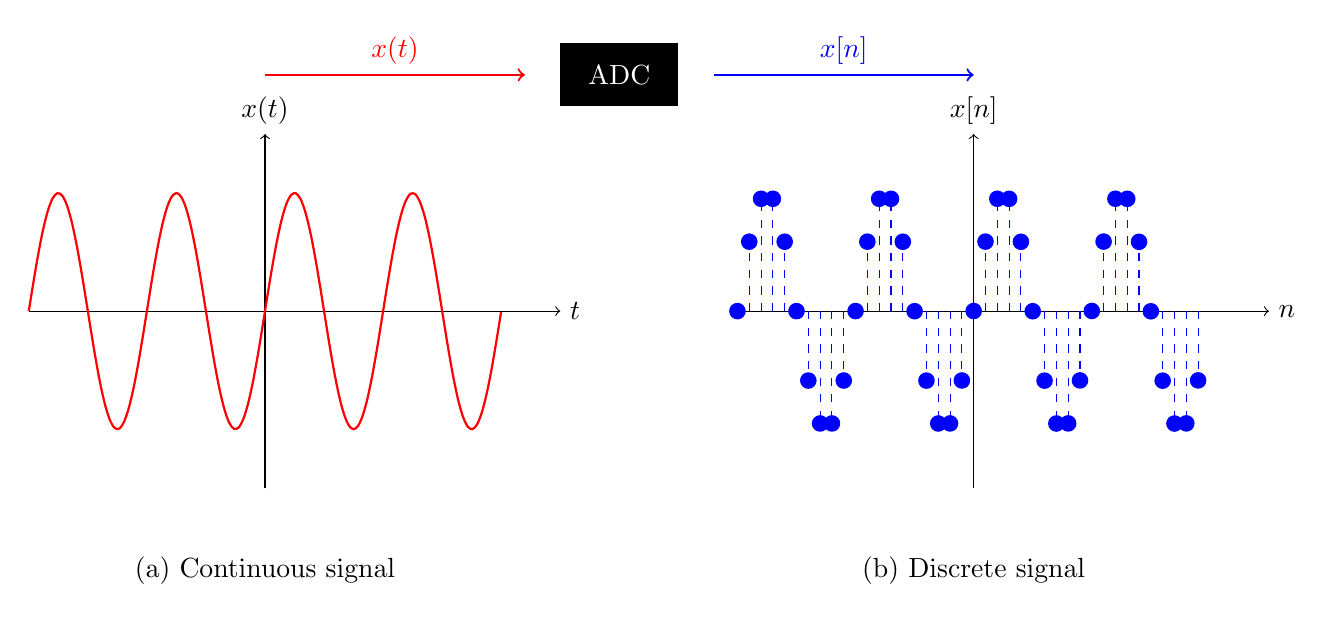
\begin{tikzpicture}[scale=1.5]
		\node[rectangle, fill=black, text=white, minimum width=1.5cm, minimum height=0.8cm] at (3,2) {ADC};
		\draw[->, thick, red] (0,2) -- (2.2,2) node[midway, above] {\color{red}$x(t)$};
		\draw[->, thick, blue] (3.8,2) -- (6,2) node[midway, above] {\color{blue}$x[n]$};
		\begin{scope}[xshift=0cm]
			\draw[->] (-2,0) -- (2.5,0) node[right] {$t$};
			\draw[->] (0,-1.5) -- (0,1.5) node[above] {$x(t)$};
			
			\draw[thick, red, smooth, domain=-2:2, samples=100] 
				plot (\x, {sin(2*180*\x)});
			
			
			\node[below] at (0,-2) {(a) Continuous signal};
		\end{scope}

		\begin{scope}[xshift=6cm]
			\draw[->] (-2,0) -- (2.5,0) node[right] {$n$};
			\draw[->] (0,-1.5) -- (0,1.5) node[above] {$x[n]$};
			
			\foreach \x in {-2,-1.9,...,2} {
				\draw[dashed, blue] (\x,0) -- (\x,{sin(2*180*\x)});
				\fill[blue] (\x,{sin(2*180*\x)}) circle (2pt);
			}
			
			
			\node[below] at (0,-2) {(b) Discrete signal};
		\end{scope}
	\end{tikzpicture}
	\caption[Analogue-to-digital conversion process]{Analogue-to-digital conversion process. The left side shows the analogue signal $x(t)$, which is sampled at discrete time intervals to produce the digital signal $x[n]$ on the right side. The dashed vertical lines indicate the sampling instants.}
	\label{fig:adc_process}
\end{figure}
In the digital domain, as illustrated on the right side of Figure \ref{fig:adc_process}, the signal is represented at discrete time intervals, each separated by a sampling period. This process is referred to as sampling. The sampling period and the sampling frequency are inversely related, as indicated in Eq. \ref{eq:sampling_frequency}

\begin{equation}
	\nu_s = \frac{1}{T_s}
	\label{eq:sampling_frequency}
\end{equation}

where $\nu_s$ is the sampling frequency, and $T_s$ is the sampling period. The sampling frequency\footnote{The term sampling rate is also commonly used and is synonymous with sampling frequency.} is typically expressed in Hz or SPS (samples per second).


The selection of an appropriate sampling frequency is determined by the frequency content of the signal under analysis. An insufficient sampling rate results in the loss of critical information and an inaccurate digital representation, mainly due to aliasing, an effect that will be discussed in more detail \S \ref{sec:nyquist_shannon}. In the other hand, an excessively high rate increases computational demands without yielding significant benefits. Achieving an optimal balance is essential in digital signal processing applications, such as spectrometry, to ensure accurate spectral analysis without introducing aliasing or unnecessary noise. The following section addresses the Nyquist-Shannon sampling theorem, which formalizes the criteria for proper sampling.

\subsection{Nyquist-Shannon sampling theorem}
\label{sec:nyquist_shannon}
The minimum sampling frequency required to prevent aliasing is defined by the Nyquist–Shannon sampling theorem, originally proposed by \citet{Nyquist1928} and later formalized by \citet{Shannon1949}. This theorem states that a baseband, bandlimited signal must be sampled at a rate greater than twice its highest frequency component to ensure all spectral information is preserved. A \emph{baseband} signal occupies frequencies near 0~Hz, while a \emph{bandpass} signal lies within a range away from 0~Hz, as in most modulated systems. Both are considered bandlimited if their spectral energy is confined within a finite bandwidth. Mathematically, the sampling condition can be expressed as
\begin{equation}
\nu_s > 2\nu_{\text{max}} ,
\label{eq:nyquist_condition}
\end{equation}
where $\nu_s$ is the sampling frequency and $\nu_{\text{max}}$ the maximum signal frequency.

The theorem extends naturally to bandpass signals, where the bandwidth $B = \nu_H - \nu_L$ is the difference between the highest and lowest frequency components. If the sampling frequency satisfies
\begin{equation}
\nu_s > 2B = 2(\nu_H - \nu_L),
\end{equation}
the signal can be fully reconstructed even when centered far above baseband. This property underlies the principle of \emph{bandpass sampling}, which deliberately exploits aliasing to translate higher-frequency content into a lower Nyquist zone.

In this context, the frequency spectrum is divided into consecutive Nyquist zones of width $\nu_s/2$: the first from 0 to $\nu_s/2$, the second from $\nu_s/2$ to $\nu_s$, and so on (see Figure~\ref{fig:nyquist_zones}). A tone in a higher Nyquist zone will appear “folded” into a lower one depending on its position relative to these boundaries. Formally, the aliased frequency $\nu_{\text{alias}}$ can be expressed as
\begin{equation}
\nu_{\text{alias}} =
\begin{cases}
\nu_{\text{tone}} \bmod \nu_\text{Nyquist} + \nu_0, & \text{for even zones},\\
\nu_\text{Nyquist} - (\nu_{\text{tone}} \bmod \nu_\text{Nyquist}) + \nu_0, & \text{for odd zones},
\end{cases}
\end{equation}
where $\nu_\text{Nyquist} = \nu_s/2$ and $\nu_0$ is the lower frequency limit of the zone.


\begin{figure}[h!]
	\centering
	\begin{tikzpicture}[scale=1.4]
		\draw[thin, dashed] (1.2,0) -- (1.2,2.5);
		\draw[thin, dashed] (2.4,0) -- (2.4,2.5);
		\draw[thin, dashed] (3.6,0) -- (3.6,2.5);
		\draw[thin, dashed] (4.8,0) -- (4.8,2.5);
		\draw[thin, dashed] (6.0,0) -- (6.0,2.5);

		\node[below] at (0,-0.1) {$0$};
		\node[below] at (1.2,-0.1) {$0.5\nu_s$};
		\node[below] at (2.4,-0.1) {$\nu_s$};
		\node[below] at (3.6,-0.1) {$1.5\nu_s$};
		\node[below] at (4.8,-0.1) {$2\nu_s$};
		\node[below] at (6.0,-0.1) {$2.5\nu_s$};

		\fill[gray!30] (0,0) rectangle (1.2,2.5);
		\fill[gray!30] (2.4,0) rectangle (3.6,2.5);
		\fill[gray!30] (4.8,0) rectangle (6.0,2.5);

		\fill[gray!60] (1.2,0) rectangle (2.4,2.5);
		\fill[gray!60] (3.6,0) rectangle (4.8,2.5);

		\node[black, align=center, font=\small\bfseries] at (0.6,1.25) {1st\\Nyquist\\Zone};
		\node[black, align=center, font=\small\bfseries] at (1.8,1.25) {2nd\\Nyquist\\Zone};
		\node[black, align=center, font=\small\bfseries] at (3.0,1.25) {3rd\\Nyquist\\Zone};
		\node[black, align=center, font=\small\bfseries] at (4.2,1.25) {4th\\Nyquist\\Zone};
		\node[black, align=center, font=\small\bfseries] at (5.4,1.25) {5th\\Nyquist\\Zone};
		\node[black, align=center, font=\small\bfseries\itshape] at (6.75,1.25) {Upper\\Nyquist\\Zones...};

		\draw[-Stealth, black, thick] (6.5,0.6) -- (7.2,0.6);

		\draw[thick, -Stealth] (0,0) -- (7.5,0) node[right] {frequency};
		\draw[thick, -Stealth] (0,0) -- (0,2.5);
	\end{tikzpicture}
	\caption[Nyquist zones]{Illustration of Nyquist Zones. Only signals in the 1st Nyquist Zone can be directly represented without aliasing. Signals in higher zones are folded into the 1st zone due to aliasing.}
	\label{fig:nyquist_zones}
\end{figure}

When $\nu_s$ is insufficient, higher-frequency components fold into the first Nyquist zone, producing spectral overlap and distortion, a phenomenon known as \emph{aliasing}. Understanding this mapping between zones is therefore essential when designing sampling systems, particularly in quadrature sampling architectures such as those employed in CHARTS.

\subsection{Quadrature sampling}
\label{sec:quadrature_sampling}
Quadrature sampling is a technique used to digitize a band-limited signal by shifting its spectrum so that it is centered at 0 Hz. Unlike conventional (real-valued) Nyquist sampling, quadrature sampling produces a complex-valued signal. In this representation, the sampling rate equals the signal bandwidth ($\nu_s = B$), meaning each complex sample contains the information of two real samples. This approach allows the representation of both positive and negative frequency components. To convert a real, Nyquist-sampled signal $x[n]$ centered at 0 Hz into a quadrature-sampled signal, it can be multiplied by a complex exponential $e^{\mathrm{j}2\pi \nu_0 n}$, resulting in
\begin{equation}
	\label{eq:quadrature_sampling}
	x'[n] = x[n] e^{\mathrm{j}2\pi \nu_0 n}
\end{equation}
where $\nu_0$ is the center frequency of the signal. This multiplication shifts the spectrum of $x[n]$ to be centered at $\nu_0$, allowing it to be sampled at a rate equal to its bandwidth. The resulting complex signal can be represented as:
\begin{equation}
	x'[n] = x_I[n] + \mathrm{j} x_Q[n]
	\label{eq:complex_signal}
\end{equation}
where $x_I[n]$ and $x_Q[n]$ represent the in-phase and quadrature components, respectively. In practice, this is implemented using a \gls{nco}, where a cosine wave is used for the in-phase component and a sine wave (90° phase-shifted) for the quadrature component, as illustrated in Figure \ref{fig:quadrature_sampling}.
\begin{figure}[h!]
	\centering
	\begin{tikzpicture}
	% Paths, nodes and wires:
	\draw (7, 5) to[sinusoidal voltage source, l_={$\cos(2\pi \nu_0n)$}] (7, 4);
	\node[mixer] at (7.01, 6){};
	\node[mixer] at (7, 1.49){};
	\node[shape=rectangle, draw, line width=1pt, minimum width=0.965cm, minimum height=0.965cm](N1) at (7, 3){} node[anchor=center] at (N1.text){$90^\circ$};
	\draw[-latex] (7, 2.5) -| (7, 2);
	\draw[-latex] (7, 5) -- (7, 5.5);
	\draw[-latex] (7, 4) -- (7, 3.5);
	\node[shape=rectangle, minimum width=1.131cm, minimum height=0.631cm] at (8, 4.5){} node[anchor=center, align=center, text width=0.743cm, inner sep=6pt] at (8, 4.5){NCO};
	\node[shape=rectangle, minimum width=1.923cm, minimum height=0.631cm] at (5.221, 3){} node[anchor=center, align=center, text width=1.535cm, inner sep=6pt] at (5.221, 3){$\sin(2\pi\nu_0 n)$};
	\node[shape=rectangle, draw, line width=1pt, minimum width=1.131cm, minimum height=0.631cm] at (8.583, 1.5){} node[anchor=center, align=center, text width=0.743cm, inner sep=6pt] at (8.583, 1.5){LPF};
	\node[shape=rectangle, draw, line width=1pt, minimum width=1.131cm, minimum height=0.631cm] at (8.583, 6){} node[anchor=center, align=center, text width=0.743cm, inner sep=6pt] at (8.583, 6){LPF};
	\node[shape=rectangle, minimum width=1.131cm, minimum height=0.631cm] at (10.583, 6){} node[anchor=center, align=center, text width=0.743cm, inner sep=6pt] at (10.583, 6){$x_I[n]$};
	\node[shape=rectangle, minimum width=1.131cm, minimum height=0.631cm] at (10.583, 1.5){} node[anchor=center, align=center, text width=0.743cm, inner sep=6pt] at (10.583, 1.5){$x_Q[n]$};
	\node[shape=rectangle, minimum width=1.131cm, minimum height=0.631cm] at (3.083, 3.667){} node[anchor=center, align=center, text width=0.743cm, inner sep=6pt] at (3.083, 3.667){$x[n]$};
	\draw[-latex] (4, 4) -- (4, 1.5) -- (6.5, 1.5);
	\draw[-latex] (7.5, 1.5) -- (8, 1.5);
	\draw[-latex] (7.5, 6) -- (8, 6);
	\draw[-latex] (9.167, 6) -- (10, 6);
	\draw[-latex] (9.167, 1.5) -- (10, 1.5);
	\draw (4, 4) -| (4, 6);
	\draw[-latex] (4, 6) -- (6.5, 6);
	\draw (3.583, 3.667) -- (4, 3.667);
\end{tikzpicture}
	\caption[Quadrature sampling block diagram]{Quadrature sampling block diagram, where a real-valued signal $x[n]$ is mixed with a cosine and sine wave at frequency $\nu_0$ to produce the in-phase ($x_I[n]$) and quadrature ($x_Q[n]$) components. The 90° phase shifter ensures the sine wave is in quadrature with the cosine wave. Digital low-pass filters (LPF) remove high-frequency components resulting from the mixing process.}
	\label{fig:quadrature_sampling}
\end{figure}

\subsection{Quantization}
\label{sec:quantization}
Quantization is the process by which the continuous amplitudes of an analogue signal are mapped to a finite set of discrete levels (the second block in the ADC present in Figure \ref{fig:heterodyne_receiver}). For an $N$-bit converter, the number of quantization levels is $L = 2^N$, and the quantized signal can be expressed as

\begin{equation}
	\hat{x}[n] = \text{round}\!\left(\frac{x[n]}{\Delta}\right)\Delta,
\end{equation}

where $\Delta = 2A / 2^N$ is the step size for an input range $[-A, A]$. This rounding introduces quantization noise, which can be modeled as a uniform random variable in $[-\Delta/2, \Delta/2]$, with average power

\begin{equation}
	P_q = \frac{\Delta^2}{12} = \frac{A^2}{3 \cdot 2^{2N}}.
\end{equation}

Increasing $N$ reduces $P_q$, but at the cost of higher data rates and storage requirements. Importantly, quantization is nonlinear: it distorts waveforms, alters frequency content, and biases statistical measures such as correlations. In radio interferometry, this leads to systematic errors and bias in both amplitude and phase, ultimately affecting source brightness and position estimates \citep{menaparra2018quantizationbiasdigitalcorrelators}.  

These issues are critical in radio astronomy, where weak celestial signals coexist with strong \gls{rfi}. To avoid clipping when the input exceeds the ADC range, high dynamic range is required. The theoretical dynamic range of an $N$-bit ADC is

\begin{equation}
	\text{DR}_{\text{ideal}} = 6.02N + 1.76 \ \text{dB}.
\end{equation}

Real devices, however, are limited by nonidealities such as jitter and thermal noise. Their performance is better described by the effective number of bits (ENOB), obtained from the measured signal-to-noise-and-distortion ratio (SINAD):

\begin{equation}
	\text{ENOB} = \frac{\text{SINAD} - 1.76}{6.02}.
\end{equation}

Another key metric is the \gls{sfdr}, which compares the fundamental tone to the largest spurious component. This is particularly relevant for mitigating intermodulation products caused by strong interferers.  

Finally, ADC outputs are often expressed in dBFS (decibels relative to full scale), where 0~dBFS corresponds to the maximum representable amplitude. In this scale, the quantization noise floor of an ideal $N$-bit converter is at approximately $-6.02N - 1.76$~dBFS.  

In summary, quantization defines the fundamental sensitivity of digital receivers. While theoretical models describe the trade-off between resolution and noise, practical evaluation requires considering ENOB, SINAD, SFDR, and dBFS, which together capture the real performance of ADCs in the presence of noise and \gls{rfi}.

\subsection{Discrete Fourier transform}
\label{sec:dft}
A large portion of signal processing is devoted to the problems of detection and estimation. Detection refers to deciding whether a particular signal set is present in the observation, while estimation concerns determining the parameters that describe it. In practice, observed signals are often corrupted by noise or interference, making these tasks non-trivial. A common strategy is to represent the signal in terms of a basis set that spans the signal space \citep{helstrom1968statistical}. For periodic signals, frequently encountered in engineering problems and radio astronomy, the natural basis consists of sines and cosines, leading directly to Fourier analysis.

\begin{figure}[h!]
	\centering
	\includegraphics[width=0.9\textwidth]{../figures/fourier_series-011.png}
	\caption[Fourier decomposition of a square periodic signal]{Fourier decomposition of a square periodic signal. The signal in the time domain (left) can be represented as the sum of sinusoidal components of different frequencies and amplitudes (center). In the frequency domain (right), each harmonic corresponds to a discrete spectral line at multiples of the fundamental frequency $1/T$. Adapted from \href{https://tikz.net/fourier_series/}{TiKz.net}, Izaak Neutelings.}
	\label{fig:fourier_decomposition}
\end{figure}

Figure~\ref{fig:fourier_decomposition} illustrates this principle. A periodic time-domain signal (left) is expressed as a linear combination of sinusoidal functions at harmonically related frequencies. Each component contributes with a specific amplitude $b_n$, shown in the frequency domain (right) as discrete spectral lines located at multiples of the fundamental frequency $1/T$. This visualization emphasizes the duality between the time and frequency domains: while the time-domain signal may appear complex, its harmonic content can be concisely described by a small set of Fourier coefficients. This spectral representation is the foundation of many detection and estimation techniques in signal processing, as it isolates the periodic components embedded in noisy or corrupted observations.

In digital implementations, we typically work with $N$ uniformly spaced samples of the observed signal. The \gls{dft} produces $N$ equally spaced samples of the corresponding periodic spectrum, offering an elegant framework for spectral decomposition in an $N$-dimensional orthogonal vector space \citep{Cooley1969finite}. Its mathematical formulation is given by

\begin{equation}
X[k] = \sum_{n=0}^{N-1} x[n] e^{-\mathrm{j} 2 \pi k n / N}, \quad k = 0, 1, \ldots, N-1,
\end{equation}
where $X[k]$ are the DFT coefficients, $x[n]$ are the input samples and $e^{-\mathrm{j} 2 \pi k n / N}$ are the basis functions.

It is important to note that the DFT operates on finite sequences, whereas its ideal counterpart, the \gls{dtft}, is defined for infinite sequences. The \gls{dtft} is expressed as:
\begin{equation}
X(\nu) = \sum_{n=-\infty}^{\infty} x[n] e^{-\mathrm{j} 2\pi\nu n}, \quad -1/2 \leq \nu < 1/2,
\end{equation}
where $X(\nu)$ is a continuous function of the frequency variable $\nu$. The DFT can be interpreted as a sampled version of the \gls{dtft}, evaluated at discrete frequency points $\nu_k = k / N$.

While the DFT provides a rigorous framework for spectral analysis, its direct computation has $\mathcal{O}(N^2)$ complexity, making it computationally expensive for large datasets. The fast Fourier transform algorithm (detailed in \S\ref{sec:fft}) reduces this to $\mathcal{O}(N \log N)$, enabling real-time processing in radio astronomy applications. 

\subsection{The fast Fourier transform}
\label{sec:fft}
The DFT can be computed efficiently by a family of algorithms collectively known as the \Gls{fft}, which reduce the arithmetic cost from $\mathcal{O}(N^2)$ to $\mathcal{O}(N\log_2 N)$ \citep{CooleyTukey1965,OppenheimSchafer2010}.

A canonical radix-2 decimation-in-time (DIT) step splits the $N$-point DFT into two $N/2$-point DFTs of the even and odd samples, which are then combined through butterfly operations:
\begin{align}
X[k] &= X_e[k] + w_N^k\, X_o[k],\\
X[k+\tfrac{N}{2}] &= X_e[k] - w_N^k\, X_o[k], \qquad k=0,\dots,\tfrac{N}{2}-1,
\end{align}
where $w_N \triangleq e^{-\mathrm{j}2\pi/N}$, and $X_e[k]$ and $X_o[k]$ denote the $N/2$-point DFTs of even and odd inputs, respectively. Figure \ref{fig:fft_algorithm} illustrates this process. The decimation-in-frequency (DIF) form applies a dual factorization on the outputs; both lead to $\log_2 N$ stages of length-2 butterflies and twiddle multiplications.

\begin{figure}[h!]
	\centering
		\begin{tikzpicture}[c/.style={circle,fill, minimum size=4pt, 
						inner sep=0pt, outer sep=0pt}]
	\foreach \i [count=\xe from 0, count=\xo from 4, 
			evaluate={\ni=int(2*\i)}, evaluate={\nii=int(\ni+1)} ] in {0,1,2,3}{%
		\draw[-] (0,-\xe*0.75cm) coordinate (xe-\xe) -- 
				node [above]{$X_e[\xe]$} ++(0:2cm) coordinate[c] (xe-\xe-1);
		\draw[-] (xe-\xe-1)--++(0:2cm) coordinate[c, label=right:{$X[\xe]$},               
				label={[font=\scriptsize]below:{$w_8^\xe$}}] (xe-\xe-2);
		\draw[-] (-2cm,-\xe*0.75cm) coordinate (xe-\xe-0)--
				++(0:-1cm)node[left]{$x[\ni]$}; 
		\begin{scope}[yshift=-4cm]
		\draw[-] (0,-\xe*0.75cm) coordinate (xo-\xe)--node [above]{$X_o[\xe]$} 
				++(0:2cm) coordinate[c] (xo-\xe-1);
		\draw[-] (xo-\xe-1)--++(0:2cm) coordinate[c, label=right:{$X[\xo]$}, 
				label={[font=\scriptsize]below:{$w_8^\xo$}}] (xo-\xe-2);
		\draw[-] (-2cm,-\xe*0.75cm) coordinate (xo-\xe-0)--
				++(0:-1cm)node[left]{$x[\nii]$}; 
		\end{scope}
	}
	\node[fit=(xe-0-0) (xe-3), draw, inner ysep=5mm, inner xsep=0pt, align=center]
			{N/2\\ DFT};
	\node[fit=(xo-0-0) (xo-3), draw, inner ysep=5mm, inner xsep=0pt, align=center]
			{N/2\\ DFT};

	\foreach \i in {0,1,2,3}{
		\draw (xe-\i -1) -- (xo-\i-2);
		\draw (xo-\i -1) -- (xe-\i-2);
	}
	\end{tikzpicture}
	\caption[FFT algorithm schematic]{Schematic representation of the FFT algorithm for $N=8$. The input signal is divided into even and odd components, which are then processed separately before being combined to produce the final output.}
	\label{fig:fft_algorithm}
\end{figure}

For streaming hardware, pipelined radix architectures organize these stages so that one sample can be accepted each clock once the pipeline is filled. Two widely used forms are the single-path delay-feedback (R2SDF) and the multi-path delay-commutator (R2MDC) pipelines. Design issues include scaling/rounding for fixed-point, twiddle scheduling and data ordering (bit-reversed vs.\ natural order\citealt{Parsons2009}). These FFT engines are the workhorses of real-time spectrometers and correlators in radio astronomy.


\subsection{Window functions and spectral leakage}
The \gls{fir} filtering stage serves to attenuate frequency components outside the desired band. Without this filtering, out-of-band signals can introduce unwanted noise within the passband due to spectral leakage and scalloping loss effects associated with the DFT applied in subsequent processing steps \citep{HUANG202061}.

Spectral leakage arises due to the finite duration of the impulse response window used in the DFT. When the transform is performed without attenuating out-of-band frequency components, it is equivalent to multiplying the signal by a rectangular window whose width matches the length of the DFT. This operation in the time domain corresponds to convolution with a sinc function in the frequency domain, as illustrated in Figure~\ref{fig:rectangular_fourier}. The result is that energy from frequencies outside the desired band \emph{leaks} into the passband, distorting the spectral estimate. Applying appropriate filtering or windowing before the DFT mitigates this effect by suppressing unwanted frequency components \citep{Price2016spectrometers}.
\begin{figure}[h!]
	\centering
	\begin{tikzpicture}
		% Parameters for both plots
		\def\xmin{-0.7*\T} % min x axis
		\def\xmax{3.0}     % max x axis
		\def\ymin{-0.4}    % min y axis
		\def\ymax{1.7}     % max y axis
		\def\A{0.67*\ymax} % amplitude
		\def\T{0.31*\xmax} % period

		% RECTANGULAR FUNCTION (LEFT SIDE)
		\begin{scope}[xshift=-4cm]
		  \draw[->,thick] (0,\ymin) -- (0,\ymax) node[left] {$x(t)$};
		  \draw[->,thick] (-\xmax,0) -- (\xmax+0.1,0) node[below,right] {$t$};
		  \draw[xline,very thick,line cap=round]
			({-\T},{\A}) -- ({\T},{\A}) node[black,right=0,scale=0.9] {$A$}
			({-\T},0) -- ({-0.9*\xmax},0)
			({ \T},0) -- ({0.9*\xmax},0);
		  \draw[xline,dashed,thin,line cap=round]
			({-\T},0) --++ (0,{\A})
			({ \T},0) --++ (0,{\A});
		  \tick{{ -\T},0}{90} node[right,below,scale=1] {$-T$};
		  \tick{{  \T},0}{90} node[right,below,scale=1] {$T$};
		\end{scope}

		% ARROW WITH FOURIER TRANSFORM SYMBOL
		\draw[<->,ultra thick,black] (-1.5,0.8) -- (1.5,0.8);
		\node[black,above] at (0,0.8) {$\mathcal{F}$};

		% RECTANGULAR FUNCTION - frequency domain (RIGHT SIDE)
		\begin{scope}[xshift=4cm]
		  \draw[->,thick] (0,\ymin) -- (0,\ymax) node[left] {$X(\omega)$};
		  \draw[->,thick] (-\xmax,0) -- (\xmax+0.1,0) node[below,right] {$\omega$};
		  \draw[xline,samples=80,smooth,variable=\t,domain=-0.94*\xmax:0.94*\xmax]
			plot(\t,{\A*sin(360/(\T)*\t)/(2*pi)*(\T)/\t});
		\end{scope}
	\end{tikzpicture}
	\caption[Fourier transform of a rectangular pulse]{Fourier transform of a rectangular pulse. The time-domain rectangular function $x(t)$ (left) is transformed into a sinc function $X(\omega)$ in the frequency domain (right).}
	\label{fig:rectangular_fourier}
\end{figure}
This can be understood if we consider that the DFT of a finite-length signal $x[n]$ can be written as
\begin{equation}
	X[k] = \sum_{n=0}^{N-1} x[n] e^{-\mathrm{j} 2\pi n k / N}
\end{equation}
which is equivalent to applying \gls{dtft} to the product of $x[n]$ and a rectangular (or tophat) window function $\Pi_N[n]$:
\begin{equation}
	X[k] = \mathcal{F}_N \left( \Pi_N[n] x[n] \right)
\end{equation}
where
\begin{equation}
	\Pi_N[n] =
	\begin{cases}
		1 & 0 \leq n \leq N-1 \\
		0 & \text{otherwise}
	\end{cases}
\end{equation}
The rectangular window is Fourier paired with the sinc function, so the finite length of the DFT effectively convolves the ideal Fourier transform (or \gls{dtft}) $X(\nu)$ with a sinc function. The undesirable peaks of the sinc function are referred to as \emph{sidelobes}.

Windowing functions improve the response of a DFT by mitigating sidelobe levels at the expense of increasing the channel width. They are applied by multiplying the signal $x[n]$ by a weighting function $w[n]$:
\begin{equation}
	X_w[k] = \sum_{n=0}^{N-1} w[n] x[n] e^{-\mathrm{j} 2\pi n k / N} = W[k] * X[k]
\end{equation}
Window functions are also fundamental in digital filter design. Among the most widely used windows in digital spectrometry are the Hamming and Hann windows, which offer a good compromise between sidelobe suppression and spectral resolution. Table \ref{tab:window_functions} lists some of the most common window functions along with their mathematical expressions. 

\begin{table}[h!]
	\centering
	\begin{tabular}{ll}
		\toprule
		\textbf{Window} & \textbf{Expression} \\
		\midrule
		Rectangular & $w[n] = 1$ \\
		Hanning & $w[n] = 0.5 - 0.5 \cos\left(\frac{2\pi n}{N-1}\right)$ \\
		Hamming & $w[n] = 0.54 - 0.46 \cos\left(\frac{2\pi n}{N-1}\right)$ \\
		Blackman & $w[n] = 0.42 - 0.5 \cos\left(\frac{2\pi n}{N-1}\right) + 0.08 \cos\left(\frac{4\pi n}{N-1}\right)$ \\
		Gaussian & $w[n] = e^{-\frac{1}{2} \left(\frac{n - (N-1)/2}{\sigma (N-1)/2}\right)^2}$ \\
	\end{tabular}
	\caption{Common window functions used in digital signal processing.}
	\label{tab:window_functions}
\end{table}




% \begin{figure}
% 	\centering
% 	\includegraphics[width=\textwidth]{tikz figures/build/fir_filter}
% 	\caption{Diagram of an 8 tap FIR filter implemented using a shift-register architecture. The input signal $x[n]$ propagates through a chain of flip-flops (FF1 to FF7), each representing a delay of $z^{-1}$. At each stage, the delayed signal is multiplied by a coefficient $h_k$, and the products are summed to generate the output $y[n]$. }
% \end{figure}

\subsection{Polyphase filter banks}
As discussed earlier, applying a window function before the DFT is a common method to reduce spectral leakage. However, this approach alone is insufficient in real-time digital spectrometers, where both efficiency and spectral purity are critical. The \gls{pfb} technique provides an elegant solution by combining windowing and decimation with the DFT in a computationally efficient way \citep{Harris1978}.

In a PFB, instead of feeding the DFT directly with $N$ samples, a longer block of length $M = N \times P$ is considered, where $P$ is the number of taps. This block is multiplied by a window function $w[n]$, often derived from a sinc function further tapered by a smoother function (e.g., Hanning or Hamming) to improve sidelobe suppression. The weighted block is then decomposed into $N$ polyphase sub-filters of length $P$, which are summed to form a filtered sequence. Finally, this sequence is processed by an $N$-point DFT, yielding spectral estimates with strongly reduced leakage.

The weighting/windowing can be thought of as a filtering process in which the elements of the window function are the filter coefficients. Mathematically, this process is given by
\begin{equation}
    h[n + pN], \quad p = 0,1,\ldots,P-1,
\end{equation}
where each sub-filter corresponds to a phase-shifted, decimated version of the prototype filter. Collectively, the $N$ sub-filters followed by the DFT stage constitute the PFB. This structure is sometimes referred to \textit{windowed pre-sum FFT}, highlighting its equivalence to overlapping windowed FFT methods but with improved implementation efficiency. Figure \ref{fig:pfb_diagram} illustrates the architecture of a PFB with $N$ channels and $P=3$ taps.

\begin{figure}[h!]
	\centering
	\begin{tikzpicture}[font=\footnotesize]
	% Paths, nodes and wires:
	\node[shape=rectangle, draw, line width=1pt, dash pattern={on 1pt off 4pt}, minimum width=9.215cm, minimum height=4.965cm] at (8.875, 4){};
	\draw (2.844, 5) to[cute closing switch] (3.75, 5);
	\node[shape=rectangle, minimum width=0.715cm, minimum height=0.715cm] at (2.125, 5){} node[anchor=north west, align=left, text width=0.327cm, inner sep=6pt] at (1.75, 5.375){$x[n]$};
	\draw (2.5, 5) -- (2.844, 5);
	\node[shape=rectangle, draw, line width=1pt, minimum width=0.965cm, minimum height=0.715cm] at (8, 5.5){} node[anchor=north west, align=left, text width=0.577cm, inner sep=6pt] at (7.5, 5.875){$z^{-1}$};
	\node[mixer] at (6.5, 3.99){};
	\node[mixer] at (9.5, 4.01){};
	\node[mixer] at (12.5, 4.01){};
	\node[ocirc] at (3.75, 5.5){};
	\node[shape=rectangle, draw, line width=1pt, minimum width=0.965cm, minimum height=0.715cm] at (11, 5.5){} node[anchor=north west, align=left, text width=0.577cm, inner sep=6pt] at (10.5, 5.875){$z^{-1}$};
	\draw[-latex] (3.75, 5.5) -- (7.5, 5.5);
	\draw[-latex] (8.5, 5.5) -- (10.5, 5.5);
	\draw[-latex] (9.5, 5.5) -- (9.5, 4.5);
	\draw[-latex] (6.5, 5.5) -- (6.5, 4.5);
	\node[shape=rectangle, minimum width=0.965cm, minimum height=0.715cm] at (4.75, 4){} node[anchor=north west, align=left, text width=0.577cm, inner sep=6pt] at (4.25, 4.375){$h[2N]$};
	\draw[-latex] (5.5, 4) -- (6, 4);
	\node[shape=rectangle, minimum width=0.965cm, minimum height=0.715cm] at (8, 4){} node[anchor=north west, align=left, text width=0.577cm, inner sep=6pt] at (7.5, 4.375){$h[N]$};
	\node[shape=rectangle, minimum width=1.215cm, minimum height=0.715cm] at (6.875, 5.875){} node[anchor=north west, align=left, text width=0.827cm, inner sep=6pt] at (6.25, 6.25){$x[2N]$};
	\node[shape=rectangle, minimum width=0.965cm, minimum height=0.715cm] at (9.5, 5.875){} node[anchor=north west, align=left, text width=0.577cm, inner sep=6pt] at (9, 6.25){$x[N]$};
	\draw[-latex] (8.5, 4) |- (9, 4);
	\draw[-latex] (11.5, 4) -- (12, 4);
	\node[shape=rectangle, minimum width=0.965cm, minimum height=0.715cm] at (11.25, 4){} node[anchor=north west, align=left, text width=0.577cm, inner sep=6pt] at (10.75, 4.375){$h[0]$};
	\draw[-latex] (11.5, 5.5) -- (12.5, 5.5) -- (12.5, 4.5);
	\node[adder] at (12.5, 2.51){};
	\draw[-latex] (12.5, 3.52) -- (12.5, 3);
	\draw[-latex] (9.5, 3.52) -- (9.5, 2.5) -- (12, 2.5);
	\draw[-latex] (6.5, 3.5) -- (6.5, 1.75) -- (12.5, 1.75) -- (12.5, 2);
	\node[shape=rectangle, minimum width=2.465cm, minimum height=0.715cm] at (5.5, 1.875){} node[anchor=north west, align=left, text width=2.077cm, inner sep=6pt] at (4.25, 2.25){Sub-filter 0};
	\node[shape=rectangle, minimum width=0.965cm, minimum height=0.715cm] at (12.5, 5.875){} node[anchor=north west, align=left, text width=0.577cm, inner sep=6pt] at (12, 6.25){$x[0]$};
	\node[ocirc] at (3.75, 4){};
	\node[shape=rectangle, draw, line width=1pt, dash pattern={on 1pt off 4pt}, minimum width=9.608cm, minimum height=4.965cm] at (8.679, -1.5){};
	\node[shape=rectangle, draw, line width=1pt, minimum width=0.965cm, minimum height=0.715cm] at (8, 0.02){} node[anchor=north west, align=left, text width=0.577cm, inner sep=6pt] at (7.5, 0.395){$z^{-1}$};
	\node[mixer] at (6.5, -1.49){};
	\node[mixer] at (9.5, -1.47){};
	\node[mixer] at (12.5, -1.47){};
	\node[shape=rectangle, draw, line width=1pt, minimum width=0.965cm, minimum height=0.715cm] at (11, 0.02){} node[anchor=north west, align=left, text width=0.577cm, inner sep=6pt] at (10.5, 0.395){$z^{-1}$};
	\draw[-latex] (4, 0.02) -- (7.5, 0.02);
	\draw[-latex] (8.5, 0.02) -- (10.5, 0.02);
	\draw[-latex] (9.5, 0.02) -- (9.5, -0.98);
	\draw[-latex] (6.5, 0.02) -- (6.5, -0.98);
	\node[shape=rectangle, minimum width=1.845cm, minimum height=0.715cm] at (4.69, -1.5){} node[anchor=north west, align=left, text width=1.457cm, inner sep=6pt] at (3.75, -1.125){$h[2N+1]$};
	\node[shape=rectangle, minimum width=1.84cm, minimum height=0.715cm] at (7.813, -1.5){} node[anchor=north west, align=left, text width=1.452cm, inner sep=6pt] at (6.875, -1.125){$h[N+1]$};
	\node[shape=rectangle, minimum width=2.09cm, minimum height=0.715cm] at (6.25, 0.375){} node[anchor=north west, align=left, text width=1.702cm, inner sep=6pt] at (5.187, 0.75){$x[2N+1]$};
	\node[shape=rectangle, minimum width=1.715cm, minimum height=0.715cm] at (9.625, 0.375){} node[anchor=north west, align=left, text width=1.327cm, inner sep=6pt] at (8.75, 0.75){$x[N+1]$};
	\draw[-latex] (8.5, -1.5) |- (9, -1.48);
	\draw[-latex] (11.5, -1.48) -- (12, -1.48);
	\node[shape=rectangle, minimum width=0.965cm, minimum height=0.715cm] at (11.25, -1.48){} node[anchor=north west, align=left, text width=0.577cm, inner sep=6pt] at (10.75, -1.105){$h[1]$};
	\draw[-latex] (11.5, 0.02) -- (12.5, 0.02) -- (12.5, -0.98);
	\node[adder] at (12.5, -2.97){};
	\draw[-latex] (12.5, -1.96) -- (12.5, -2.48);
	\draw[-latex] (9.5, -1.96) -- (9.5, -2.98) -- (12, -2.98);
	\draw[-latex] (6.5, -1.98) -- (6.5, -3.73) -- (12.5, -3.73) -- (12.5, -3.48);
	\node[shape=rectangle, minimum width=2.465cm, minimum height=0.715cm] at (5.5, -3.605){} node[anchor=north west, align=left, text width=2.077cm, inner sep=6pt] at (4.25, -3.23){Sub-filter 1};
	\node[shape=rectangle, minimum width=0.965cm, minimum height=0.715cm] at (12.5, 0.395){} node[anchor=north west, align=left, text width=0.577cm, inner sep=6pt] at (12, 0.77){$x[1]$};
	\draw[-latex] (5.5, -1.5) |- (6.01, -1.49);
	\draw (3.75, 5) -- (4, 5) -| (4, 0.02);
	\node[shape=rectangle, draw, line width=1pt, minimum width=2.393cm, minimum height=4.215cm] at (16.929, 4.286){} node[anchor=center, align=center, text width=2.005cm, inner sep=6pt] at (16.929, 4.286){\Large FFT $N$ -point};
	\draw[-latex] (12.99, 2.51) -- (13.75, 2.5) -- (13.714, 5.429) |- (15.714, 5.429);
	\draw[-latex] (13, -3) -- (14, -3) -- (14, 4.714) -- (15.714, 4.714);
	\draw[-latex] (3.75, 4) -| (3.75, -5.25) -- (14.25, -5.25) -- (14.143, 3.429) -- (15.714, 3.429);
	\node[shape=rectangle, minimum width=2.965cm, minimum height=0.715cm] at (5.75, -4.875){} node[anchor=north west, align=left, text width=2.577cm, inner sep=6pt] at (4.25, -4.5){Sub-filter $N-1$};
	\node[shape=rectangle, minimum width=1.215cm, minimum height=0.715cm] at (15, 5.875){} node[anchor=north west, align=left, text width=0.827cm, inner sep=6pt] at (14.375, 6.25){$y[0]$};
	\node[shape=rectangle, minimum width=1.215cm, minimum height=0.715cm] at (15, 5.125){} node[anchor=north west, align=left, text width=0.827cm, inner sep=6pt] at (14.375, 5.5){$y[1]$};
	\node[shape=rectangle, minimum width=1.59cm, minimum height=0.715cm] at (14.938, 3.125){} node[anchor=north west, align=left, text width=1.202cm, inner sep=6pt] at (14.125, 3.5){$y[N-1]$};
	\node[shape=rectangle, minimum width=0.465cm, minimum height=0.965cm] at (3.75, 4.5){} node[anchor=north, align=center, text width=0.077cm, inner sep=6pt] at (3.75, 5){\tiny .\\.\\.};
	\node[shape=rectangle, minimum width=0.465cm, minimum height=0.965cm] at (9, -4.75){} node[anchor=north, align=center, text width=0.077cm, inner sep=6pt] at (9, -4.25){\tiny .\\.\\.};
	\node[shape=rectangle, minimum width=0.465cm, minimum height=0.965cm] at (14.938, 4){} node[anchor=north, align=center, text width=0.077cm, inner sep=6pt] at (14.938, 4.5){\tiny .\\.\\.};
\end{tikzpicture}
	\caption[Polyphase filter bank schematic]{Schematic of a PFB with three taps ($P=3$) and an $N$-point FFT. The input signal $x[n]$ is processed through $N$ sub-filters, each corresponding to a phase of the prototype filter. The outputs of these sub-filters are summed and then transformed by the FFT to produce the final spectral output. Adapted from \url{https://casper.berkeley.edu/wiki/The_Polyphase_Filter_Bank_Technique}.}
	\label{fig:pfb_diagram}
\end{figure}

Given all of this, the PFB enhances the FFT, improving spectral channel frequency response (Figure~\ref{fig:hamming_window_response}). This requires extra resources for buffering additional samples and performing complex multiplications for each filter tap.

\begin{figure}
	\centering
	\includegraphics{../figures/hamming_window_response_db.pdf}
	\caption[Comparison of single-bin frequency response between PFB and FFT]{Comparison of the single-bin frequency response of a PFB with a direct FFT. Here, the length of the polyphase window is 4 times the length of the FFT. The PFB exhibits significantly lower sidelobe levels and a sharper main lobe, resulting in improved spectral purity and reduced leakage.}
	\label{fig:hamming_window_response}
\end{figure}

\section{Spectrometers and correlators}
A spectrometer is an instrument designed to detect and quantify the spectral components of signals, such as radio waves originating from astronomical objects. It specifically measures the power spectral density (PSD, typically expressed in units of \si{\watt \per \hertz}) of a signal. Examining the spectral content provides insights into the characteristics of radio sources and the properties of the medium through which the signals travel \citep{Price2016spectrometers}.

A correlator, on the other hand, is a specialized type of spectrometer that computes the cross-correlation between signals received at different antennas in an interferometric array. In Figure~\ref{fig:correlator_schematic}, we illustrate a basic two-element interferometer setup. Each antenna captures the incoming wavefront from a distant source, converting it into an electrical signal. Due to the spatial separation between the antennas, there is a geometric time delay $\tau_g$ between the signals received at each antenna. This delay depends on the baseline vector $\mathbf{b}$ (the vector connecting the two antennas) and the direction of the incoming wavefront, characterized by the angle $\theta$. The total time delay $\tau_\text{total}$ includes both this geometric delay and any additional instrumental delays.
 

\begin{figure}[h!]
      \centering
      \begin{tikzpicture}
        \edef\d{2.5}    % distance between block
        \edef\m{-2.5}     % slope
        \edef\height{2} % height wavefront

        \coordinate (A) at (-\d, 0);
        \coordinate (B) at (\d, 0);

        \node[regular polygon,regular polygon sides=3, draw, shape border rotate=180, scale=0.5, fill=black] (Atel) at (A) {\color{white} $Y$};
        \node[regular polygon,regular polygon sides=3, draw, shape border rotate=180, scale=0.5, fill=black] (Btel) at (B) {\color{white} $X$};

        \node[rectangle, draw, fill=black] at (Atel.south) {};
        \node[rectangle, draw, fill=black] at (Btel.south) {};

        \path let \p1=(Atel.north) in (Atel.north) -- ($(\x1, \y1) + (\height / \m, \height)$) coordinate (WA);
        \path (WA) -- ++ (\d * 2, 0) coordinate (WB);

        \path[<-|, thin] ($(Atel.south) + (0, -.3)$) -- node[midway] (baseline) {$\mathbf{b}$} ($(Btel.south) + (0, -.3)$);
        \draw[<-] ($(Atel.south) + (0, -.3)$) -- (baseline);
        \draw[-|] (baseline) -- ($(Btel.south) + (0, -.3)$);


        \draw[very thin] (Atel.north) -- ($(Btel.north)!(Atel.north)!(WB)$) coordinate (Bmid);
        \draw[very thin] (Atel.north) -- ($(Bmid)!-1.5cm!(Atel.north)$) coordinate (C);
        \draw[->, thin] (Atel.north) -- ($(Bmid)!-3cm!(Atel.north)$) coordinate (D) node[above] {$R_{xy}(\tau)$};

        % tau measurement
        \coordinate (Btelright) at ($(Btel.north) + (1, 0)$);
        \path (Btelright) -- ($(Bmid)!(Btelright)!(C)$) coordinate (C1);
        
        % transparent node
        \path[<->|, thin] (C1) -- node[midway] (tau) {$\tau_\text{total}$} ($(Btelright)!(Btel.north)!(C1)$);
        \draw[<-, thin] (C1) -- (tau);
        \draw[->|, thin] (tau) -- ($(Btelright)!(Btel.north)!(C1)$);

        \draw[dashed, ultra thin] (Btel.north) --++ (-\d, 0);
        \coordinate (AN) at (Atel.north);
        \coordinate (BN) at (Btel.north);

        % angle theta
        \pic[draw, thin, <->, "$\theta$", angle eccentricity=1.3, angle radius=.8cm] {angle=Bmid--BN--AN};

		\begin{scope}[xscale=0.5, yscale=0.5, shift={(C)}, rotate={atan(\m)}]
					\draw[thick, domain=-3.5:3.5, smooth, samples=100] 
						plot (\x, {sin(deg(2*\x*pi))/(\x*pi)});
					\draw[->] (-4, 0) -- (4, 0) node[right] {$\tau$};
				\end{scope}

        \coordinate (WB2) at ($(Bmid)!-1cm!(Btel.north)$);
        \coordinate (WA2) at ($(Atel.north)!(WB2)!(WA)$);
        \draw (WB2) -- (WA2);
        %\pic[rotate={atan(-1 / \m)}] at (WA2) {wavefront};
        \path (WA2) -- node[midway, sloped, gray, above] {wavefront} (WB2);

        % adding source
        \path ($(WA)!-.5cm!(Atel.north)$) -- ($(Btel.north)!4.5cm!(WB)$) node[midway, circle, inner sep=0pt, outer sep=0pt, draw, label=\color{gray}{source}, minimum size=0.1cm, gray, fill=gray] {};

        % ($(Bmid)!(Btelright)!(C)$)
        \draw[dashed, ultra thin] (Atel.north) -- (WA);
        \draw[dashed, ultra thin] (Btel.north) -- ($(Btel.north)!4cm!(WB)$);

        \draw[->, thin] (WA2) -- ($(WA2)!-0.6cm!(Atel.north)$) node[left] {$\widehat{\mathbf{n}}$};
        \draw[->, thin] (WB2) -- ($(WB2)!-0.6cm!(Btel.north)$) node[left] {$\widehat{\mathbf{n}}$};
      \end{tikzpicture}
      \caption[The two element radio interferometer]{The two element radio interferometer. The signals received at antennas $X$ and $Y$ are cross-correlated to produce the visibility function $R_{xy}(\tau)$, which is a measure of the spatial coherence of the incoming wavefront. The time delay $\tau_\text{total}$ includes both the geometric delay $\tau_g = \mathbf{b} \cdot \widehat{\mathbf{n}} / c$ and any additional instrumental delays. The angle $\theta$ represents the direction of the incoming wavefront relative to the baseline vector $\mathbf{b}$. Adapted from \citet{Cassanelli_2022}.}
	  \label{fig:correlator_schematic}
\end{figure}

In the following subsections, we explore the theoretical foundations that underpin the operation of spectrometers and correlators, focusing on the Wiener-Khinchin theorem and its cross-correlation counterpart.
\subsection{Wiener-Khinchin theorem}
There are two primary methods for calculating the PSD, also referred to as the power spectrum, of a signal. The power spectrum, denoted as $S_{xx}$, and the autocorrelation function, $R_{xx}$, of a waveform are connected through the Wiener-Khinchin theorem. This theorem establishes that for a stationary (constant mean and variance) and ergodic (statistically consistent over time) signal $x(t)$, the PSD and autocorrelation are related by

\begin{equation}
	S_{xx}(\nu) = \int_{-\infty}^{\infty} R_{xx}(\tau) e^{- \mathrm{j} 2\pi \nu \tau} d\tau
	\label{eq:continous-wiener-khinchin}
\end{equation}

where $\nu$ represents frequency and $\tau$ denotes the time lag. The autocorrelation function of an ergodic process is defined as \citep{Gubner_2006}
\begin{equation}
	R_{xx}(\tau) =  \langle x(t) x^*(t - \tau)\rangle = \lim_{T \to \infty} \frac{1}{2T} \int_{0}^{T} x(t) x^*(t - \tau) dt
	\label{eq:continous_autocorrelation}
\end{equation}
where $^*$ denotes the complex conjugate and $\langle \cdot \rangle$ denotes the expectation value, which is the average over time for a stationary signal. For discrete signals, which are far more common in practice due to the increasing use of digital systems such as the spectrometer developed in this thesis, the theorem can be expressed as
\begin{equation}
	S_{xx}(\nu) = \sum_{m=-\infty}^{\infty} \left\langle x[n] x^*[n - m] \right\rangle e^{-\mathrm{j}2\pi m \nu}
	\label{eq:discrete-wiener-khinchin}
\end{equation}
where $m$ is the time lag index and $\nu$ is the normalized frequency in the interval $[-1/2,1/2]$. Spectrometers that calculate the PSD using Eq. \ref{eq:discrete-wiener-khinchin} are known as autocorrelation spectrometers (from now on XF ACS). These spectrometers compute the autocorrelation function of the input signal first and then apply a DTFT to obtain the PSD. Using this definition in Eq. \ref{eq:discrete-wiener-khinchin} and the convolution theorem, the PSD can also be expressed as
\begin{equation}
	S_{xx}(\nu) = \left\langle |X(\nu)|^2 \right\rangle
	\label{eq:discrete_psd}
\end{equation}
where $X(\nu)$ is the DTFT output at frequency $\nu$. This result shows that the PSD can be obtained directly by averaging the squared magnitude of the DFT output. This is significant because it enables the computation of the PSD from the DFT\footnote{Important is to clarify that the integration time must be sufficiently long to ensure that DFT and DTFT are approximately equal.} of the signal, eliminating the need to explicitly calculate the autocorrelation function which can be computationally expensive, especially for large arrays. This type of spectrometer is known as fourier transform filterbanks (from now FX FTF spectrometers). Figure \ref{fig:psd_methods} illustrates the two methods for calculating the PSD of a signal, highlighting the differences between ACS and FTF spectrometers.
\begin{figure}[h]
	\centering
	\begin{tikzpicture}[block/.style={rectangle, draw, minimum width=2cm, minimum height=1.2cm, align=center},
    arrow/.style={-{Stealth[length=3mm]}, thick},
    node distance=3cm]

	% Fila superior
	\node[block] (x1) {$x(t)$};
	\node[block, right=4cm of x1] (x2) {$x(t)x^*(t-\tau)$};
	\node[block, right=4cm of x2] (x3) {$\langle x(t)x^*(t-\tau) \rangle$};

	% Fila inferior
	\node[block, below=2cm of x1] (X1) {$X(\nu)$};
	\node[block, below=2cm of x2] (X2) {$|X(\nu)|^2$};
	\node[block, below=2cm of x3] (S) {$S_{xx}$};

	% Flechas horizontales superiores
	\draw[arrow] ([xshift=-0.5cm]x1.west) -- (x1.west);
	\draw[arrow] (x1.east) -- (x2.west) node[midway, above] {\small delay \& multiply};
	\draw[arrow] (x2.east) -- (x3.west) node[midway, above] {\small time average};

	% Flechas horizontales inferiores
	\draw[arrow] (X1.east) -- (X2.west) node[midway, above] {\small square};
	\draw[arrow] (X2.east) -- (S.west) node[midway, above] {\small time average};

	% Flecha de salida
	\draw[arrow] (S.east) -- ([xshift=0.5cm]S.east);

	% Flechas verticales (DFT)
	\draw[arrow] (x1.south) -- (X1.north) node[midway, left] {\small DFT};
	\draw[arrow] (x3.south) -- (S.north) node[midway, right] {\small DFT};

	\end{tikzpicture}
	\caption[Methods for computing PSD]{Block diagram showing two equivalent methods for computing the PSD of a signal. The upper path represents what a ACS system does, while the lower path represents a FTF system. Adapted from \citet{Price2016spectrometers}.}
	\label{fig:psd_methods}
\end{figure}


\subsection{Cross-correlation}
\label{sec:cross_correlation}
In radio interferometers, multiple antennas observe the same astronomical source, each recording its individual response. To derive the system's overall response, the signals from all antennas must be combined. This is accomplished by computing the cross-correlation function between pairs of signals, effectively cross-correlating the responses from different antennas.
The cross-correlation operation is often denoted by the pentagram symbol ($\star$) and is defined as:
\begin{equation}
	R_{xy}(\tau)=\left[x(t) \star y(t)\right](\tau) = \lim_{T \to \infty} \frac{1}{2T} \int_{-T}^{T} x(t) y^*(t - \tau) dt
\end{equation}
This integral can also be expressed as a convolution:
\begin{align}
	\left[x(t) \star y(t)\right](\tau) 
	&= \int_{-\infty}^{\infty} x(t)\, y^*(t - \tau)\, dt \\
	&= \int_{-\infty}^{\infty} x(t)\, y^*(-(\tau - t))\, dt \\
	&= \left[x(t) * y^*(-t)\right](\tau)
	\label{eq:cross_correlation}
\end{align}
where $y^*(-t)$ denotes the time-reversed and conjugated version of $y(t)$. Applying the Fourier transform to both signals, and using the convolution theorem, we obtain:
\begin{equation}
	x(t) \star y(t) \xrightarrow{\mathcal{F}} X(\nu) Y^*(\nu)
	\label{eq:cross_correlation_fourier}
\end{equation}
where $X(\nu)$ and $Y(\nu)$ are the Fourier transforms of $x(t)$ and $y(t)$, respectively. The right-hand side of Eq. \ref{eq:cross_correlation_fourier}, $X(\nu) Y^*(\nu):=S_{xy}(\nu)$, is known as the cross power spectrum of $x(t)$ and $y(t)$. This result shows that the cross power spectrum is the Fourier transform of the cross-correlation function. In the special case where $X = Y$, this reduces to the Wiener–Khinchin theorem discussed previously. This relationship forms the theoretical foundation for cross-correlation spectrometry.

\subsection{Correlator architectures}
\label{sec:spectrometer_architectures}
Correlators are generally divided into two main categories. In a lag (or XF) correlator, the cross-correlation operation is performed first, followed by a Fourier transform (analogous to an ACS system). An example of radiotelescopes using this architecture is the WIDAR correlator in the \Gls{vla} \citep{Perley_2009} and \Gls{alma} correlator \citep{ALMA_correlator}.

Conversely, in an FX correlator, the Fourier transform is applied before the cross-correlation. In this type of correlator, the digitized data stream from each antenna is first transformed into a frequency spectrum using a real-time FFT. For every antenna pair, the resulting complex frequency components are then multiplied to obtain the cross power spectrum. The computational load is dominated by the Fourier transform stage, and the total number of operations scales with the number of antennas. In contrast, for a lag correlator, the computational effort is mainly determined by the number of antenna pairs. Therefore, the FX architecture is more hardware-efficient, particularly as the number of antennas increases (see Section 8.8.5 of \citealt{thompson2017interferometry}). Examples of contemporary radio telescopes employing FX correlators for FRB detection include \gls{chime} \citep{CHIME/FRB_2018}, \gls{askap} \citep{Shannon_2025}, MeerKAT \citep{MeerKAT}, Galactic Radio Explorer (GReX; \citealt{GReX}) and Bustling Universe Radio Survey (BURSTT; \citealt{BURSTT}).

Figure \ref{fig:corr_methods} illustrates the two correlator architectures, analogous to the methods for computing the PSD shown in Figure \ref{fig:psd_methods}.
\begin{figure}
	\centering
	\begin{tikzpicture}[
		block/.style={rectangle, draw, minimum width=2.5cm, minimum height=1.5cm, align=center},
		arrow/.style={-{Stealth[length=3mm]}, thick},
		node distance=2.5cm
	]
		% Top row: x(t), y(t)
		\node[block] (xtyt) {%
			$x(t)$\\
			$y(t)$
		};
		\node[block, right=5cm of xtyt] (XnuYnu) {%
			$X(\nu)$\\
			$Y(\nu)$
		};

		% Bottom row: Rxy, Sxy
		\node[block, below=2cm of xtyt] (Rxy) {%
			$R_{xy}(\tau) = $\\
			$\frac{1}{T}\int_0^T x(t)y^*(t-\tau)\,dt$
		};
		\node[block, below=2cm of XnuYnu] (Sxy) {%
			$S_{xy}(\nu) =$\\
			$X(\nu)Y^*(\nu)$
		};

		% Horizontal arrows (top)
		\draw[arrow] (xtyt.east) -- node[above, midway] {DFT} (XnuYnu.west);

		% Horizontal arrows (bottom)
		\draw[arrow] (Rxy.east) -- node[above, midway] {DFT} (Sxy.west);

		% Vertical arrows
		\draw[arrow] (xtyt.south) -- node[left, midway] {cross-correlation} (Rxy.north);
		\draw[arrow] (XnuYnu.south) -- node[right, midway] {cross-power spectrum} (Sxy.north);

	\end{tikzpicture}
	\caption[Correlator architectures]{Block diagram illustrating the two correlator architectures: XF (bottom) and FX (top). The left side represents the time-domain operations, while the right side represents the frequency-domain operations. Adapted from \citet{thompson2017interferometry}}.
	\label{fig:corr_methods}
\end{figure}
Due to the advantages of the FX architecture, the remainder of this section focuses on various implementations of FX correlators and spectrometers.
\subsection{F-engine}
In an FX correlator, the F-stage (commonly referred to as the F-engine) is responsible for three main tasks: channelization, requantization with gain adjustment and corner turn with packetization. Channelization allows for frequency-specific signal corrections, facilitates efficient distribution of data throughout the correlator hardware, and enables the cross-correlation of antenna pairs via complex multiplication.  

As illustrated in Fig.~\ref{fig:f-engine}, the input signal is first digitized by the ADC, providing a discrete representation of the analogue voltages from each antenna. The PFB and FFT perform the channelization, dividing the wideband signal into narrow frequency bins with reduced spectral leakage. 

To reduce bandwidth and storage requirements, the spectra are re-quantized to a lower bit depth while maintaining adequate sensitivity. The corner turn operation then reorganizes the data: instead of being grouped by antenna, the output is arranged by frequency channel, which is the natural format required for the cross-correlation step. Finally, the packetizer encapsulates the data into network packets for efficient transmission to the X-engine, where the correlation products are computed.

\begin{figure}[h]
	\centering
	\begin{tikzpicture}[
			block/.style={rectangle, draw, thick, minimum width=1cm, minimum height=0.8cm, align=center, fill=gray!10, font=\small},
			arrow/.style={-{Stealth[length=2.5mm]}, thick},
			node distance=0.7cm]

			% F-engine components
			\node[block] (adc) {ADC};
			\node[block, right=of adc] (pfb) {PFB};
			\node[block, right=of pfb] (fft) {FFT};
			\node[block, right=of fft] (requant) {Re-quant.};
			\node[block, right=of requant] (corner) {Corner\\ Turn};
			\node[block, right=of corner] (packet) {Packetizer};

			% Connect blocks with arrows
			\draw[arrow] (adc) -- (pfb);
			\draw[arrow] (pfb) -- (fft);
			\draw[arrow] (fft) -- (requant);
			\draw[arrow] (requant) -- (corner);
			\draw[arrow] (corner) -- (packet);
		\end{tikzpicture}
	\caption[Block diagram of the F-engine processing chain]{Block diagram of the F-engine processing chain in an FX correlator. The input signal is digitized by the ADC, then undergoes coarse delay correction, filtering through a polyphase filterbank, and transformation to the frequency domain via FFT. Fine delay adjustment and re-quantization prepare the data for the corner turn operation, which rearranges data by frequency rather than by antenna before packetization for transmission to the X-engine.}
	\label{fig:f-engine}
\end{figure}

\subsection{X-engine}
After the F-engine has channelized and packetized the data, the X-engine receives these packets, typically over high-speed network links. In modern radio telescopes, the X-engine is responsible for performing the complex cross-multiplication and accumulation of visibilities across all antenna pairs, forming the basis for imaging and calibration.
For an array with $N_\text{ant}$ antennas, the number of unique baselines is $N_\text{bsl} = N_\text{ant}(N_\text{ant}+1)/2$, leading to a computational cost per spectral frame that scales as
\begin{equation}
	\mathcal{O} !\left(N_\nu,N_\text{ant}^2\right),
\end{equation}
where $N_\nu$ is the number of frequency channels. Temporal integration only changes the multiplicative constant (the number of accumulations), not the asymptotic scaling.

In addition to correlation, X-engines can perform beamforming by coherently summing antenna voltages with appropriate delays or phase rotations. A straightforward delay-and-sum implementation for $B$ beams has a computational complexity of
\begin{equation}
\mathcal{O}!\left(N_\nu,B,N_\text{ant}\right),
\end{equation}
which becomes prohibitive for large arrays. However, for regularly sampled arrays, FFT beamforming can be applied to synthesize approximately $N_\text{ant}$ orthogonal beams with a reduced cost of
\begin{equation}
\mathcal{O}!\left(N_\nu,N_\text{ant}\log_2 N_\text{ant}\right),
\end{equation}
substantially improving efficiency when $B \sim N_\text{ant}$ \citep{Masui_2019}.
This approach, however, constrains the array geometry and pointing grid but is widely used in large-$N$, wide-field interferometers where real-time beamforming is required \citep{Price_2024}.

\section{Computational hardware}
\label{sec:computational_hardware}
The digital signal processing required by modern radio telescopes relies primarily on four platforms: \glspl{cpu}, \glspl{gpu}, \glspl{fpga}, and \glspl{asic}. Each offers different trade-offs in terms of flexibility, efficiency, and development cost.  

\begin{itemize}
	\item \Glspl{asic} are custom-designed circuits optimized for a specific task. They powered major facilities such as the JVLA and ALMA correlators \citep{Perley_2009,ALMA_correlator}. Although their fabrication is costly and inflexible, they provide unmatched power efficiency, making them attractive for large-scale projects such as the SKA \citep{D_Addario_2016}.  

	\item \Glspl{gpu}, originally developed for graphics rendering, have become widely used in high-performance computing. Their highly parallel architecture makes them ideal for large matrix operations and real-time data processing, often serving as backends for cross-correlation and imaging pipelines. An example of a pipeline specifically dedicated to \glspl{gpu} is the X-engine of \gls{chime} \citep{recnik2015efficientrealtimedatapipeline, Denman_2015}. 

	\item \Glspl{fpga} occupy a middle ground between flexibility and efficiency. They interface directly with \glspl{adc} and high-speed links, handling tasks such as channelization and packetization before passing data downstream. Their role in radio astronomy has been facilitated by open-source initiatives like \Gls{casper} \citep{hickish2016decadedevelopingradioastronomyinstrumentation}, and they remain the dominant choice for first-stage DSP. A dedicated discussion is provided in \S~\ref{sec:fpgas}. 
	\item \glspl{cpu} retain a central role as general-purpose processors. While less efficient for massively parallel tasks, they provide the control logic, coordination, and post-processing capabilities required in heterogeneous architectures that combine multiple platforms. 
\end{itemize} 

 
In practice, modern correlators employ hybrid solutions: \glspl{fpga} or \glspl{asic} for front-end channelization and packetization, followed by \glspl{gpu} or \glspl{cpu} clusters for cross-correlation and higher-level data products. This balance leverages the strengths of each technology to meet the demanding performance and scalability requirements of radio astronomy.

\subsection{Field programmable gate arrays}
\label{sec:fpgas}
\Glspl{fpga} are reconfigurable integrated circuits that offer a flexible hardware platform capable of being programmed in the field, with performance approaching that of \glspl{asic}, yet without the fabrication lead time and high cost of custom silicon \citep{kuon2008fpga}.

At their core, \Glspl{fpga} consist of a structured array of fundamental resources:
\begin{itemize}
  \item \textbf{\Glspl{clb}}, which include \glspl{lut} and registers for implementing arbitrary combinational and sequential logic.
  \item \textbf{Programmable interconnect fabric} that routes signals flexibly between CLBs and other blocks.
  \item \textbf{Dedicated specialized blocks}, such as DSP units for arithmetic operations and \glspl{bram} for efficient data storage.
  \item \textbf{I/O blocks} that interface with external signals and support a variety of standards and voltage levels.
\end{itemize}

A typical \Gls{fpga} layout can thus be visualized as a matrix of CLBs  surrounded by I/O pads and interconnected via hierarchical routing networks. Each CLB (see Figure \ref{fig:clb_structure}) usually contains multiple LUTs and flip-flops, as well as multiplexers to support flexible logic structures, including arithmetic carry chains and synchronous timing.

\begin{figure}[h!]
	\centering
	\begin{tikzpicture}
		% Paths, nodes and wires:
		\node[latch] at (6.453, 5.16){};
		\draw[line width=1pt] (9, 8.167) -- (9, 5.167) -- (10, 6.167) -- (10, 7.167) -- cycle;
		\node[shape=rectangle, draw, line width=1pt, minimum width=1.965cm, minimum height=1.965cm] at (3, 5.75){} node[anchor=center, align=center, text width=1.577cm, inner sep=6pt] at (3, 5.75){LUT};
		\node[shape=rectangle, minimum width=0.715cm, minimum height=0.465cm] at (0.946, 6.536){} node[anchor=north west, align=left, text width=0.327cm, inner sep=6pt] at (0.571, 6.786){A};
		\node[shape=rectangle, minimum width=0.715cm, minimum height=0.465cm] at (0.946, 6){} node[anchor=north west, align=left, text width=0.327cm, inner sep=6pt] at (0.571, 6.25){B};
		\node[shape=rectangle, minimum width=0.715cm, minimum height=0.465cm] at (0.946, 5.464){} node[anchor=north west, align=left, text width=0.327cm, inner sep=6pt] at (0.571, 5.714){C};
		\node[shape=rectangle, minimum width=0.715cm, minimum height=0.465cm] at (0.946, 4.964){} node[anchor=north west, align=left, text width=0.327cm, inner sep=6pt] at (0.571, 5.214){D};
		\node[shape=rectangle, minimum width=0.715cm, minimum height=0.465cm] at (9.556, 4.861){} node[anchor=north west, align=left, text width=0.327cm, inner sep=6pt] at (9.181, 5.111){S};
		\draw (9.5, 5) -- (9.5, 5.667);
		\node[shape=rectangle, minimum width=1.393cm, minimum height=0.608cm] at (11.536, 6.679){} node[anchor=north west, align=left, text width=1.005cm, inner sep=6pt] at (10.821, 7){Output};
		\draw (1.143, 6.429) -| (2, 6.4);
		\draw (1.143, 5.857) -- (2, 5.857);
		\draw (1.143, 5.286) -- (2, 5.286);
		\draw (1.143, 4.857) -- (2, 4.857);
		\node[shape=rectangle, minimum width=1.393cm, minimum height=0.608cm] at (4.8, 4.321){} node[anchor=north west, align=left, text width=1.005cm, inner sep=6pt] at (4.086, 4.643){clk};
		\draw (4, 6) -- (5.333, 6);
		\draw (10, 6.667) -| (10.905, 6.655);
		\draw (7.573, 6) -| (9, 6);
		\draw (4.8, 6) -| (4.8, 7.4) -- (9, 7.4);
		\draw (5.333, 4.32) |- (4.8, 4.321);
	\end{tikzpicture}
	\caption[CLB internal architecture]{Internal architecture (simplified) of a CLB in an FPGA. The CLB consists of LUTs for implementing Boolean functions, a memory element (typically a D-type flip-flop), and a multiplexer to used to select the data output between combinational and sequential logic. The structure may vary depending on the FPGA manufacturer and model.}
	\label{fig:clb_structure}
\end{figure}

The inclusion of specialized DSP blocks streamlines high-speed operations such as multiplication and accumulation, while block RAM provides storage far more resource-efficient than distributed logic registers. Moreover, modern FPGAs often integrate additional features such as high-speed transceivers, phase-locked loops (PLLs), and even embedded microprocessor cores or \gls{rfsoc} capabilities, enhancing their versatility for complex applications (see \citealt{zhang2018fpga}, Chapter 8).

FPGA architecture grants a compelling trade-off: designers can implement custom circuits with parallelism tailored to the application, while still retaining reconfigurability. Compared to fixed architectures like CPUs or GPUs, FPGAs achieve higher performance per watt for many tasks, especially where spatial parallelism and low-latency processing are essential \citep{kuon2008fpga,zhang2018fpga}.

\subsection{Ethernet interconnects}

Ethernet has become the standard interconnect technology in modern radio astronomy backends, providing a scalable and cost-effective solution for transporting high data rates between FPGAs, GPUs, and storage systems \citep{Price_2020}. Commercial high-speed variants such as 10~GbE, 40~GbE, and 100~GbE (QSFP28) are routinely employed, enabling real-time redistribution of digitized signals in FX correlators and spectrometers.  

A key design choice in these systems is the adoption of the \gls{udp} as the transport layer. UDP is lightweight and connectionless, avoiding the complexity and latency penalties of TCP. Since astronomical signal processing prioritizes sustained throughput over guaranteed delivery, packet loss is tolerated at a low level, with robustness ensured by packet formats that embed sufficient metadata. Typical headers include a master counter (MCNT), antenna or ADC identifier, frequency channel indices, and payload data. This design allows receiving nodes to reassemble the data stream even in the presence of dropped or out-of-order packets.  

UDP-based transmission thus enables efficient implementation of the corner turn, where data must be reorganized from time-major to frequency-major order for correlation or further spectral analysis. By leveraging Ethernet switches, this operation can be distributed across the network without requiring custom interconnects. The combination of Ethernet and UDP has therefore become a defining feature of current large-scale radio interferometers.  


\subsection{RFSoC 4x2}
\label{sec:rfsoc}

The RFSoC 4x2\footnote{\url{https://www.realdigital.org/hardware/rfsoc-4x2}}, developed by RealDigital in collaboration with AMD-Xilinx, is a heterogeneous processing platform based on the Zynq UltraScale+ RFSoC Gen3 architecture. This board integrates high-speed analog-to-digital and digital-to-analog converters directly with FPGA fabric and embedded processors, making it particularly well-suited for real-time digital signal processing and software-defined radio (SDR) applications. Figure~\ref{fig:rfsoc_top_view} presents a top view of the board and its principal components.
\begin{figure}[h!]
\centering
\includegraphics[scale=0.58]{../figures/rfsoc.png}
\caption[RFSoC 4x2 principal components]{Top view of the RFSoC 4x2 FPGA board. SMA connectors provide access to four ADCs and two DACs, while high-speed ports such as QSFP28 enable fast data offload. Extracted from the RFSoC 4x2 datasheet \citep{RealDigital_RFSoC4x2_RefMan_A3}.}
\label{fig:rfsoc_top_view}
\end{figure}
The board supports up to 5 GSPS sampling for 14-bit ADCs and up to 9.85 GSPS for 14-bit DACs, enabling wideband direct RF sampling without the need for external downconversion stages. Four ADC SMA ports and two DAC SMA ports are available, complemented by a MABA-011118 balun (10~MHz–10~GHz) that allows single-ended antenna or signal source connections with no additional circuitry. Each converter is organized into tiles: ADCs A and B belong to tile 224, ADCs C and D to tile 226, while DACs A and B are part of tiles 228 and 230, respectively. Every tile includes a PLL, clock distribution logic, and digital up/down converters (DUC/DDC) for flexible data-path configurations. Figure~\ref{fig:rfsoc_tiles} illustrates the arrangement of the ADC and DAC tiles on the board.

\begin{figure}[h!]
\centering
\includegraphics[scale=0.7]{rfsoc_tiles.png}
\caption[RFSoC4x2 ADC and DAC tiles]{RFSoC4x2 ADC and DAC tiles. The board contains two ADC and two DAC tiles, each with integrated PLLs, mixers, and digital up/down converters. A MABA-011118 balun is connected between each SMA and ADC, supporting single-ended antenna connections. Extracted from the RFSoC 4x2 datasheet \citep{RealDigital_RFSoC4x2_RefMan_A3}.}
\label{fig:rfsoc_tiles}
\end{figure}


Beyond data converters, the RFSoC 4x2 integrates a powerful FPGA fabric with 930k logic cells and 4200 DSP slices, alongside a processing system featuring a quad-core ARM Cortex-A53, a dual-core Cortex-R5F, and an ARM Mali-400 GPU. Two independent \SI{4}{GB} DDR4 memories operate at 2400~MHz, one attached to the processing system and one to the programmable logic, ensuring high-throughput data handling. Internal UltraRAM and block RAM further enhance buffering and streaming capabilities.

The board also provides multiple high-speed interfaces for data offload and system integration, including a \gls{100gbe} QSFP28 port, USB~3.0, and a Mini DisplayPort. External clock and \gls{pps} SMA ports enable precise synchronization and multi-board operation. Power regulation and monitoring are handled by dedicated ICs, with protection against overvoltage, overcurrent, and overheating.




